\documentclass[12pt]{article}
\usepackage{amsthm}
\usepackage{bbm}
\usepackage{amssymb}
\usepackage{mathtools,etoolbox,xcolor}
\usepackage{booktabs}
\usepackage{enumitem}
\usepackage{url}
\usepackage{setspace}
\usepackage[margin=1in]{geometry}
\usepackage{authblk}
\usepackage[round,sort]{natbib}
\setcitestyle{aysep={}} 
\usepackage[page]{appendix}
\usepackage[nomarkers,nolists]{endfloat}
\renewcommand{\efloatseparator}{\mbox{}}
\usepackage{subcaption}
\renewcommand{\t}[1]{\tilde{#1}}
\newcommand{\partiall}[1]{\frac{\partial}{\partial #1}}
\newcommand{\gm}{\theta}
% \newcommand{\E}{E}
\renewcommand{\P}{P}
% \newcommand{\V}{Var}
% \newcommand{\cov}{Cov}
\newcommand{\bnd}{B}
\newcommand{\A}{A}
\newcommand{\B}{B}
% \newcommand{\Bprime}{B'}
% \newcommand{\Aprime}{A'}
% \newcommand{\fbound}{b}
% \newcommand{\mindensity}{f}
% \newcommand{\thetaind}{\theta_{ind}}
\newcommand{\corr}{Corr}
\newcommand{\mean}[1]{\overline{#1}}
\newcommand{\sel}[1]{#1^*}
\newcommand{\biasratio}{r}% {$(E|S_1-S_2|)^2/\E(S^2)$}
\newcommand{\cind}{\perp \!\!\! \perp}
\newtheorem{theorem}{Theorem}
\newtheorem{proposition}[theorem]{Proposition}
\newtheorem{lemma}[theorem]{Lemma}
\newtheorem{corollary}[theorem]{Corollary}
\newcommand{\z}{Z}
\newcommand{\y}{Y}
\newcommand{\s}{S}
\newcommand{\w}{W}
\newcommand{\x}{X}
\renewcommand{\u}{U}
\renewcommand{\v}{V}
\newcommand{\zvec}{\vec{Z}_n}
\newcommand{\svec}{\vec{S}}
\renewcommand{\vec}[1]{\textbf{#1}}
\newcommand{\Svec}{\vec{R}}
\newcommand{\eval}{\lambda}
\newcommand{\evec}{\vec{v}}
\newcommand{\thetahat}{\hat{\theta}}
\newcommand{\h}[2]{\{(\u_{#1}-\u_{#2})(\v_{#1}-\v_{#2})>0\}}
\newcommand{\zs}[2]{\frac{\z_{#1}-\z_{#2}}{\s_{#1}-\s_{#2}}}
\newcommand{\ol}[1]{\overline{#1}}
\DeclareMathOperator{\supp}{supp}
\DeclareMathOperator{\diag}{diag}
\DeclareMathOperator{\E}{E}
\DeclareMathOperator{\V}{Var}
\DeclareMathOperator{\Var}{Var}
\DeclareMathOperator{\Cov}{Cov}
% \DeclareMathOperator{\diag}{diag}
% \DeclareMathOperator{\x}{x}
% \DeclareMathOperator{\theta4}{\hat{\theta4}}
% \DeclareMathOperator{\thetaind}{\hat{\theta}_{\cind}}
% \DeclareMathOperator{\mindensity}{p}
% \DeclareMathOperator{\bnd}{r}
% \DeclareMathOperator{\A}{A}
% \DeclareMathOperator{\B}{B}
% \DeclareMathOperator{\Aprime}{A'}
% \DeclareMathOperator{\Bprime}{B'}
% \DeclareMathOperator{\f0bound}{p}
% \DeclareMathOperator{\C}{C}
\mathtoolsset{showonlyrefs=true}
\newtoggle{commenttoggle}
\newcommand{\comment}[1]{
  \iftoggle{commenttoggle}{
    {\normalsize{\color{red}{ #1}}\normalsize}
  }
  {}
}

\togglefalse{commenttoggle}
\doublespace
\title{A Correction to Begg's Test for Publication Bias}
\author[1]{Haben Michael}
\author[2]{Musie Ghebremichael}
\affil[1]{University of Massachusetts, Amherst, MA (hmichael@math.umass.edu)}
\affil[2]{Ragon Institute and Harvard University, Cambridge, MA (musie\_ghebremichael@dfci.harvard.edu)}
\date{}                   
\begin{document}
\maketitle

\noindent \textsc{Summary}: Begg and Mazumdar proposed using a rank
correlation test to test for publication bias when carrying out
meta-analyses. The asymptotic variance of the rank correlation test
statistic was derived under assumptions unmet by this application,
often resulting in a loss of power. Low power when Begg's test is used
to screen for publication bias may lead to false positives in a
subsequent meta-analysis. We obtain the asymptotic bias under the
common conditionally normal model as a function of the distribution of
primary study variances. In simulations we consider the performance of
Begg's test using an approximation to the correct asymptotic
variance. We consider this performance under the common fixed effects
and random effects frameworks. We then examine several meta-analyses
drawn from the literature where the standard and
bias-corrected versions of Begg's test lead to different conclusions.\\
\textsc{Keywords}: Publication bias; Meta-analysis; Error rates;
Kendall's tau.

% \begin{enumerate}
\section{Introduction}
  % \begin{enumerate}
  % \item meta-analysis, publication bias, tests for publication bias

  Meta-analysis is a popular technique for summarizing a body of
  studies. Key to the soundness of the approach is that the body of
  studies used in forming the summary be representative of the studies conducted. This
  requirement may fail to be met when publication bias is present, that is,
  when the availability of a study is tied to its findings \citep{begg1994b}. Several
  hypothesis tests have been proposed with the goal of identifying the
  presence of publication bias on the basis of the relationship
  between the conclusion of the study and various study
  characteristics.
  
  Common to these tests is that the null is held to be no publication
  bias. A typical conservative analyst might be expected to treat the
  presence of publication bias as the null. Given the manifold sources
  of publication bias, devising a test under such a null does not
  appear practical. The result of taking the null to be the absence of
  publication bias, however, is that Type II errors in the test for
  publication bias will often correspond to Type I errors in the
  subsequent meta-analysis. Assessing and improving the power of the
  screening test is therefore worthwhile.

  One of the most common tests for publication bias, Begg's test
  \citep{begg1994a}, tests for correlation between the studies' reported
  effect sizes and their standard errors.  An issue with Begg's test
  procedure is that it uses the asymptotic variance for a general
  correlation test derived under assumptions unmet by Begg's
  test. This nominal variance is often larger than the correct
  variance, as discussed below. As a result, the test does not reject
  as frequently as it ought, which, as mentioned above, is likely to
  lead to Type I error in the meta-analysis for which the publication
  bias test is being performed.

    
  % \item beggs test, problem with test, significance of problem for
    % publication bias

    
    
    
  % \item preview computation of magnitude of error [proposed solution?]. differentiate from bergen paper.

  This issue with Begg's test has been noted previously, including by
  the author of the test \citep{begg1994a,begg1994b}. More recently,
  \citet{gjerdevik2014} showed that the observations forming the input
  to the rank correlation test are correlated, so that the usual
  assumptions for the test are not met. Since the
  rank correlation test depends on an asymptotic approximation, this
  criticism isn't entirely fair unless the effect of the correlation
  does not vanish in the limit, as we show.

  The remainder of the paper is organized as follows. In Sections
  \ref{section:theory:begg description} and \ref{section:theory:source
    of bias}, we describe Begg's test in greater detail and identify
  the source of bias. In \ref{section:theory:direction} we discuss the
  direction of the bias and relate it to the error rates of the test,
  and in Section \ref{section:theory:gaussian} we present the form of
  the bias in the normal model assumed by \citet{begg1994a}. In
  Section \ref{section:simulations}, we contrast the power of Begg's
  test as standardly used and a debiased version, using simulated
  data. In Section \ref{section:data analysis}, we examine three
  meta-analyses drawn from biomedical literature in which the standard
  and debiased versions of Begg's test, applied in a hypothesis
  testing framework, offer diverging conclusions.
  
  % \end{enumerate}
  \section{Asymptotic bias of Begg's test}
  \label{section:theory}
\subsection{Description of test}
\label{section:theory:begg description}
% \begin{enumerate}
  % \item intro begg's test, logic of begg's test, problem with
    % correlation
    % section: description of beggs test
    
    Begg's test is a test of correlation between the reported effect
    sizes and their reported variances. The premise is that a tendency
    to publish larger effect sizes induces a trend in effect sizes
    across their variances, and no such trend exists without
    selection. See Fig. \refeq{fig:selection} for an illustration.
    
    The data consists of independent pairs
    $(\y_1,\sigma_1),\ldots,(\y_n,\sigma_n),$ representing the estimated
    effect sizes and sampling variances of $n$ studies with a common mean effect size, say $\theta$:
    \begin{align}
      \begin{split}
      \E(\y_j\mid\sigma_j)=\theta, j=1,\ldots,n\\
      \V(\y_j\mid\sigma_j^2)=\sigma_j^2.
      \label{model:nonpara}
    \end{split}
    \end{align}
    The null is that $\y_j$ is uncorrelated with $\sigma_j$, $j=1,\ldots,n$.
    % Given study effects $y_1,\ldots,y_n$ assumed normal
    % with variances $\sigma_1^2,\ldots,\sigma_n^2$ and common mean
    % $\mu$.[does theorem 1 hold when mu isnt 0? yes kernel doesnt
    % depend on translation] 
    The test statistic is Kendall's rank
    correlation coefficient,
    $$
    \hat\tau=2{n\choose 2}^{-1}\sum_{j<k}\left\{(\u_j-\u_k)(\v_j-\v_k)>0\right\} - 1,
    $$
    applied to the sequence of pairs $(\u_j,\v_j)$ given by the data after standardizing the effect sizes,
    \begin{align}
      \begin{split}\label{defn:pairs}
        (\u_j,\v_j)&=\left(\frac{\y_j-\hat{\theta}}{\sqrt{\sigma_j^2-\sigma^2_{\hat{\theta}}}},\sigma_j\right),j=1,\ldots,n,\\
        \text{where}\\
        \hat{\theta}&=(\sum_{j=1}^n\y_j/\sigma^2_j)/(\sum_{j=1}^n1/\sigma_j^2),\\
        \sigma^2_{\hat{\theta}}&=1/\sum_{j=1}^n(1/\sigma_j^2).
      \end{split}
    \end{align}
    % where[[mention dependence of u on n, $u^{(n)}_j$]]
    The mean estimate
    $\hat{\theta}=(\sum_{j=1}^n\y_j/\sigma^2_j)/(\sum_{j=1}^n1/\sigma_j^2)$
    is the inverse-variance weighted estimate of the common study mean
    $\theta$ and $\sigma^2_{\hat{\theta}}=1/\sum_{j=1}^n(1/\sigma_j^2)$
    is its variance, both conditional on the study variances.  The
    test statistic counts the number of corresponding pairs of
    studentized effect sizes
    $\u_j=(\y_j-\hat{\theta})/\sqrt{\sigma_j^2-\sigma^2_{\hat{\theta}}}$
    and variances $\v_j=\sigma_j$ that concord in
    the sense that either $\u_j<\u_k$ and $\v_j<\v_k$ or $\u_j>\u_k$ and
    $\v_j>\v_k$. The null of no correlation is to be interpreted as no
    publication bias, and is rejected at level $\alpha$ when
    $\sqrt{9n/4}|\hat\tau| > \Phi^{-1}(1-\alpha/2)$. %  [U-statistic with
    % kernel ... .]

    The asymptotic null variance $4/9$ is derived under the assumption
    that the pairs form an IID sequence. This assumption does not hold
    for the pairs (\refeq{defn:pairs}) due to the common terms
    $\hat{\theta}$ and $\sigma^2_{\hat{\theta}}$. While the latter is
    of order $1/n$ and typically negligible in the limit, the
    dependence induced by the summary statistic $\thetahat$,
    ordinarily of order $1/\sqrt{n}$, must be accounted for in
    computing the asymptotic null variance of $\sqrt{n}\hat\tau$.
    
    % to the fixed-effects summary statistics $\hat{\theta}$ and fixed effects variances $1/\sum_j\sigma_j^{-2}$ common to all the pairs.
  % \item theorem--true asymptotic null variance
  %   \begin{enumerate}
  %   \item assumptions--IID, normal response
  %     \item if discussing power, also inroduce alternative models
  %   \end{enumerate}
  % \end{enumerate}
    
  \subsection{Source of bias}\label{section:theory:source of bias}
  
  The variance of $\sqrt{n}\hat\tau$ is 
    \begin{align}
      % \Cov(\sqrt{n}\tau)=4n{n\choose 2}^{-2}\sum_{1\le i,j,k,l\le n}\Cov(\h{i}{j},\h{k}{l})
      \V(\sqrt{n}\hat\tau)=4n{n\choose 2}^{-2}\sum_{i<j,k<l}\Cov(\h{i}{j},\h{k}{l}).
    \end{align}% \comment{display should say var instead of cov. also summation should be over i<j, k<l, to match definition of tau above}
    The sum has ${n\choose 2}{n-2\choose 2}$ terms where $i,j,k,l$ are
    all distinct, $6{n\choose 3}$ terms where the set
    $\{i,j,k,l\}$ has size 3, and ${n\choose 2}$ terms where
    $|\{i,j,k,l\}|=2$:
    \begin{align}
      \V(\sqrt{n}\hat\tau)&=4\frac{(n-2)(n-3)}{n-1}\Cov(\h{1}{2},\h{3}{4})\\
      &\hspace{2em}+16\frac{n-2}{n-1}\Cov(\h{1}{2},\h{1}{3}) + O(1/n).
    \end{align}    
     The second term on the right-hand side, with the $O(1)$ coefficient, converges in probability to
    % $$16\cdot\Cov\left(\left\{\left(\frac{\y_1-\thetahat}{\sigma_1}-\frac{\y_2-\thetahat}{\sigma_2}\right)(\sigma_1-\sigma_2)>0\right\},\left\{\left(\frac{\y_1-\thetahat}{\sigma_1}-\frac{\y_3-\thetahat}{\sigma_3}\right)(\sigma_1-\sigma_3)>0\right\}\right) = 4/9,$$
    \begin{align}
    16\cdot\Cov&\left(\left\{\left(\frac{\y_1-\theta}{\sigma_1}
          -\frac{\y_2-\theta}{\sigma_2}\right)(\sigma_1-\sigma_2)>0\right\} ,
                 \left\{\left(\frac{\y_1-\theta}{\sigma_1}-\frac{\y_3-\theta}{\sigma_3}\right)(\sigma_1-\sigma_3)>0\right\}\right)\\
      &=4/9,
    \end{align}
    the usual asymptotic variance of
    Kendall's $\tau$ under the  null that $U_j$ and $V_j$ are independent, $j=1,\ldots,n.$
    % [details:
    % \begin{align}
    %   \P&((u_1-u_2)(v_1-v_2)>0,(u_1-u_3)(v_1-v_3)>0)=\\
    %     &= \P(u_1>u_2,u_1>u_3)\P(v_1>v_2,v_1>v_3) +\\
    %       &2\P(u_1>u_2,u_1<u_3)\P(v_1>v_2,v_1<v_3)+\\
    %      &\P(u_1<u_2,u_1<u_3)\P(v_1<v_2,v_1<v_3)\\
    %    &=2\E(F_{U}^2)^2 + 2(\E(F_U(U)(1-F_U(U))))^2 = 2((1/12+1/4)^2 + (1/2-1/12+1/4)^2)=5/18
    % \end{align}
    % so $16\Cov_{1213}=16(5/18-1/4)=4/9$.
    % ]
    % \begin{align}
    %   &\P((u_1-u_2)(v_1-v_2)>0,(u_1-u_3)(v_1-v_3)>0)=\\
    %   &6+6=3
    % \end{align}
    The first term on the right-hand side, with an $O(n)$ coefficient, is a
    source of bias if the covariance
    \begin{align}
      &\Cov(\h{1}{2},\h{3}{4})=\\ 
      &\hspace{2em}\Cov\left(\left\{\left(\frac{\y_1-\thetahat}{\sqrt{\sigma_1^2-\sigma_{\thetahat}^2}}
        -\frac{\y_2-\thetahat}{\sqrt{\sigma_2^2-\sigma_{\thetahat}^2}}\right)(\sigma_1-\sigma_2)>0\right\} ,
       \left\{\left(\frac{\y_3-\thetahat}{\sqrt{\sigma_3^2-\sigma_{\thetahat}^2}}-\frac{\y_4-\thetahat}{\sqrt{\sigma_4^2-\sigma_{\thetahat}^2}}\right)(\sigma_3-\sigma_4)>0\right\}\right)
        \label{eqn:cov_bias_source}
    \end{align}
    does not vanish faster than $1/n$. The false positive rate of
    Begg's test will exceed or fall below the nominal level when the
    direction of the bias is negative or positive, respectively, i.e., when the covariance (\refeq{eqn:cov_bias_source}) is positive or negative.

    \subsection{Direction of bias}
    \label{section:theory:direction}
    % Ignore variance estimate.

    Shifting the data if necessary, assume in (\refeq{model:nonpara})
    that the common mean $\theta$ is $0$, and suppose that $\y_j/\sigma_j$
    has a fixed distribution, say $F_Z$, i.e., 
    $\y_1,\ldots,\y_n$ belong to a scale
    family. % May rewrite the data as
    % $(\z_1,\sigma_1),\ldots,(\z_n,\sigma_n)$, where $z_j=y_j/\sigma_j$
    % and $z_j$ is independent of $\sigma_j$, $j=1,\ldots,n$.
    Lemma \ref{lemma:sigma_theta term} states that the $O(1/n)$ terms $\sigma_{\thetahat}^2$  in (\refeq{defn:pairs}) may often be ignored
    under this assumption. While the condition on the density of $Z$
    excludes some common densities that diverge quickly, e.g.,
    symmetric beta distributions with common shape parameter
    $\le 1/2$, it is required anyway for the general result \eqref{eqn:general variance} presented
    below.
    \begin{lemma}\label{lemma:sigma_theta term}
      Given pairs $(\y_1,\sigma_1),\ldots,(\y_n,\sigma_n)$ such that
      $\z_j=\y_j/\sigma_j,j=1,\ldots,n,$ are IID, assume
    \begin{enumerate}
      \item there are $b,B\in\mathbbm{R}$ such that
        $ 0 < b < \frac{1}{n}\sum_{j=1}^n1/\sigma_j^2 < B < \infty,$
        \item $\sigma_1,\ldots,\sigma_n,$ are distinct, and
      \item $\int_{-\infty}^\infty f_\z(z)^2dz < \infty$.
      \end{enumerate}
      Then conditional on $\sigma_1,\ldots,\sigma_n$,
      \begin{align}
        \left|{n\choose 2}^{-1}\sum_{j<k}\left\{\left(\frac{\y_j-\hat\theta}{\sigma_j}-\frac{\y_k-\hat\theta}{\sigma_k}\right)(\sigma_j-\sigma_k)>0\right\} - \hat\tau\right| = o_P(n^{-1/2}).
      \end{align}
    \end{lemma}


    Besides the scale family assumption, suppose
    further that $F_Z$ is the distribution of a symmetric random
    variable. Let $\s^2=1/\sigma^2$ denote the study precisions. In summary,
    \begin{align}
      \begin{split}
        \label{model:symmetric}
        \z_1,\ldots,\z_n &\overset{IID}{\sim} F_Z\\
        \s_1,\ldots,\s_n &\overset{IID}{\sim}  F_S\\
        \z_j &\sim -\z_j,\\
        \z_j \mid \s_j &\sim \z_j,\\
        \y_j&=\z_j/\s_j,j=1,\ldots,n.
      \end{split}
    \end{align}
% Ignoring the $O(1/n)$ terms $\sigma_{\thetahat}^2$ in (\refeq{defn:pairs}), 
The test statistic may be written in terms of $\z$ and $\s$ as
    \begin{align}
      \hat\tau=\sum_{j<k}\left\{\frac{\z_j-\z_k}{\s_j-\s_k}>\thetahat\right\}.
    \end{align}
    The covariance (\ref{eqn:cov_bias_source}) determining the bias of the asymptotic variance relative to $9/4$ is
    \begin{align}
      % \Cov\left(\left\{\frac{\z_1-\z_2}{\s_1-\s_2}>\thetahat\right\},\left\{\frac{\z_3-\z_4}{\s_3-\s_4}>\thetahat\right\} \right).
      \Cov\left(\left\{\zs{1}{2}>\thetahat\right\},\left\{\zs{3}{4}>\thetahat\right\} \right).
    \end{align}
    The grand mean estimate $\thetahat=\sum_j \z_j\s_j/\sum \s_j^2$ % is a function of
    % $(\z_1,\s_1),\ldots,(\z_n,\s_n)$ and
    induces dependence
    between the two terms in the covariance. By the symmetry of $F_Z$, $\P(\{\frac{z_j-z_k}{s_j-s_k}>\thetahat\}=1/2$, so the last expression is
    \begin{align}
     \E\left(\left\{\zs{1}{2}>\thetahat\right\}\left\{\zs{3}{4}>\thetahat\right\}\right)-1/4
     =\P\left(\zs{1}{2}\wedge\zs{3}{4}>\thetahat\right)-1/4.
    \end{align}    
    The symmetry of $F_Z$ further implies that $\{\zs{1}{2}>\thetahat\}\{\zs{3}{4}>\thetahat\}$ has the same distribution as $\{\zs{1}{2}<\thetahat\}\{\zs{3}{4}<\thetahat\}$, so the condition for a positive bias, $\E(\{\zs{1}{2}>\thetahat\}\{\zs{3}{4}>\thetahat\})<1/4$, is
      % has the same distribution as
      % $\{\x < \thetahat\}\{\y < \thetahat\}$, so the problem is the
      % same as showing [break up following. there are multiple
      % inequalities/equalities so it isnt clear which one 'the problem'
      % refers to]
      \begin{align}
        1/2 &> \P\left(\left\{\zs{1}{2}>\thetahat\right\}\left\{\zs{3}{4}>\thetahat\right\}\right) + \P\left(\left\{\zs{1}{2}<\thetahat\right\}\left\{\zs{3}{4}<\thetahat\right\}\right)\\
        % \P(\{\x > \thetahat\}\{\y > \thetahat\}) + \P(\{\x < \thetahat\}\{\y < \thetahat\}) = \P((\x-\thetahat)(\y-\thetahat) > 0)\\
        % 1/2 &> \P(\{\x > \thetahat\}\{\y > \thetahat\}) + \P(\{\x < \thetahat\}\{\y < \thetahat\}) = \P((\x-\thetahat)(\y-\thetahat) > 0)\\
            % &= \P(\x\y - \thetahat(\x + \y) + \thetahat^2 > 0)\\
            &\hspace{2em}= \P(\zvec^T(\Svec_1\Svec_2^T+\Svec_2\Svec_1^T)\zvec/2>0),
      \end{align}
      where $\zvec=(\z_1,\ldots,\z_n)$ and (for $n\ge 5$)

      \begin{align}
        \Svec_1&=\left(\frac{\sum\s_j^2}{\s_1-\s_2}-\s_1, \frac{-\sum\s_j^2}{\s_1-\s_2}-\s_2,-\s_3,\ldots,-\s_n\right)/ \sum\s_j^2  \\
        \Svec_2&=\left(-\s_1,-\s_2,\frac{\sum \s_j^2}{\s_3-\s_4}-\s_3, \frac{-\sum \s_j^2}{\s_3-\s_4}-\s_4,-\s_5,\ldots,-\s_n\right)/ \sum \s_j^2.\\
        % \Svec_1&=(\frac{1}{\s_1-\s_2}-\frac{\s_1}{\sum\s_j^2}, \frac{-1}{\s_1-\s_2}-\frac{\s_2}{\sum\s_j^2},\frac{-\s_3}{\sum \s_j^2},\ldots,\frac{-\s_n}{\sum \s_j^2})  \\
        % \Svec_2&=(-\frac{\s_1}{\sum \s_j^2},\frac{-\s_2}{\sum \s_j^2},\frac{1}{\s_3-\s_4}-\frac{\s_3}{\sum\s_j^2}, \frac{-1}{\s_3-\s_4}-\frac{\s_4}{\sum\s_j^2},-\frac{\s_5}{\sum \s_j^2},\ldots,\frac{-\s_n}{\sum \s_j^2}).
      \end{align}
      The two nonzero eigenvalues of $(\Svec_1\Svec_2^T+\Svec_2\Svec_1^T)/2$ are $\eval_a\pm\eval_b$ where
      \begin{align}
        \eval_a&=-1/(2\sum_j\s_j^2)\\
        \eval_b&=\frac{\sqrt{((\s_1-\s_2)^2/\sum_j\s_j^2-2)((\s_3-\s_4)^2/\sum_j\s_j^2-2)}}{2(\s_1-\s_2)(\s_3-\s_4)}.
      \end{align}
      % Then $\eval_a-\eval_b\le 0 \le \eval_a+\eval_b$, and
      % $|\eval_a+\eval_b|<|\eval_a-\eval_b|$,
      Then $|\eval_a|<|\eval_b|$,
      $\eval_a-|\eval_b|<0<\eval_a+|\eval_b|$, so one eigenvalue is
      negative and the other positive, while
      $|\eval_b| - \eval_a> |\eval_b|+ \eval_a,$ so the negative
      eigenvalue is larger in magnitude. Let $\evec_1,\evec_2$ denote
      unit eigenvectors associated respectively to the positive and
      negative eigenvalues. The condition for a positive bias takes
      the form
      \begin{align}
        \P\left( -\frac{\eval_a}{\eval_b} > \frac{\zvec^T(\evec_1^{\otimes 2}-\evec_2^{\otimes 2})\zvec}{\zvec^T(\evec_1^{\otimes 2}+\evec_2^{\otimes 2})\zvec} \right) > 1/2.\label{eqn:iff_cond}
      \end{align}

      The ratio $-\eval_a/\eval_b$ is $>0$ of order $1/n$. A
      sufficient condition for a positive bias is then
      $\P(\zvec^T(\evec_1^{\otimes 2}-\evec_2^{\otimes 2})\zvec<0)\ge 1/2$
      or
      \begin{align}
        \P(|\zvec^T\evec_1|<|\zvec^T\evec_2|)\ge 1/2.\label{eqn:suff_cond}
      \end{align}
      The projections $\zvec^T\evec_1,\zvec^T\evec_2$ are uncorrelated
      with mean zero. When $\z$ is gaussian, they are IID
      conditionally on $\s$, and (\refeq{eqn:suff_cond}) holds with
      equality. In general, however, whether (\refeq{eqn:iff_cond}) %  or
      % (\refeq{eqn:suff_cond})
      holds, and therefore whether the bias is positive or negative,
      depends on the distributions of $\z$ and of $\s$. Whether the
      bias is positive or negative, in turn, determines whether the
      Type II or Type I error rate of Begg's test is
      inflated. Fig. \ref{fig:negative bias} presents the results of a
      small simulation where the data exhibit negative bias.

      % Though the focus here is on a positive bias, both for the
      % reasons discussed in the Introduction and because of the
      % centrality of the gaussian case in meta-analyses,
      % Fig. \ref{fig:negative bias} presents the results of a small
      % simulation where the data exhibit negative bias. The study
      % distribution $F_Z$ is taken to be a symmetric beta distribution
      % shifted to be centered at the origin. The simulation suggests
      % that FPR control is lost as the distribution becomes
      % bimodal. Moreover, not only does the test become inconsistent,
      % but the error rate increases with the size of the
      % meta-analysis. In terms of the foregoing discussion, the
      % covariance (\ref{eqn:cov_bias_source}) does not vanish. A
      % similar situation occurs when $F_Z$ is taken to be Student's t
      % distribution as the degrees of freedom approach $1$.[[this example doesnt make sense because the variance of such t is undefined]]

      % These examples are useful in suggesting that negative test bias
      % is related to lesser mass at the center of the distribution than
      % the extremes. They are, however, far from the the gaussian case
      % for which the test was developed \citep{begg1994a}. In fact, the
      % Student's t cases that cause trouble have infinite variances, so
      % that the basic meta-analysis model \eqref{model:nonpara} does
      % not hold.


      
      \subsection{Bias in the gaussian model}
      \label{section:theory:gaussian}
    The study effects are often modeled as gaussian by appealing to
    the CLT, e.g., in the original paper \citet{begg1994a}. In this
    situation, the bias takes the form given by Theorem \ref{theorem:1}.
    \comment{proofs to appendix depending on journal}
    \begin{theorem}\label{theorem:1}
      Given pairs $(\y_j,\sigma_j),j=1,\ldots,n$, such that
      \begin{enumerate}
      \item $(\y_1,\ldots,\y_n)|(\sigma_1,\ldots,\sigma_n)\sim
      N(0,\diag(\sigma_1^2,\ldots,\sigma_n^2)),$ and
    \item for $p=1,2$, $\lim_{n\to\infty}n^{-1}\sum_{i=1}^n\sigma_i^{-p}$ exists and is finite.
    \end{enumerate}
    Then,
      \begin{align}
        \V(\sqrt{n}\hat\tau)\to 4/9 - \frac{\left(\lim {n\choose 2}^{-2}\sum_{i<j}|1/\sigma_i-1/\sigma_j|\right)^2}
        {\pi \lim n^{-1}\sum 1/\sigma_i^2}.
      \end{align}      
\end{theorem}

\begin{corollary}\label{corollary:1}
  Given IID pairs $(\y_j,\sigma_j),j=1,\ldots,n$, such that
      $(\y_1,\ldots,\y_n)|(\sigma_1,\ldots,\sigma_n)\sim
      N(0,\diag(\sigma_1^2,\ldots,\sigma_n^2)),$
      $\s>0$ a.s., $\s$ has a
      continuous density, $\E(\s^2)<\infty$, and $F_{\s}$ is H\"older continuous at $0$, i.e., $P(S\le s)$ is $O( s^\epsilon)$  for some $\epsilon>0$, then
      $\V(\sqrt{n}\hat\tau)\to 4/9 - \frac{(\E|\s_1-\s_2|)^2}{\pi\E(\s^2)}$.
    \end{corollary}

    % \begin{theorem}\label{theorem:1} Given IID $(\y_j,\s_j),j=1,\ldots,n$, such that
    %   $$(\y_1,\ldots,\y_n)|(\s_1,\ldots,\s_n)\sim
    %   N(0,\diag(1/\s_1^2,\ldots,1/\s_n^2)),$$ $\s>0$ a.s., $\s$ has a
    %   continuous lebesgue density, $\E(\s^2)<\infty$, and $P(S^2\le s)$ is $O( s^\epsilon)$  for some $\epsilon>0$, then
    %   $\V(\sqrt{n}\tau)\to 4/9 - \frac{(\E|\s_1-\s_2|)^2}{\pi\E(\s^2)}$.
    % \end{theorem}
    For a general distribution for the
    response $\z$, in many typical cases, the
    limiting variance is
    \begin{align}
    4/9 - \frac{4(\E|\s_1-\s_2|)^2}{E(\s^2)}\E(f_\z(\z))(2\E(\z F_\z(\z))-\E(f_\z(\z))).\label{eqn:general variance}
    \end{align}
    This result follows by exploiting the theory of U-processes
    \citep{nolan1988}. The proof given here for the gaussian case in Theorem
    \ref{theorem:1} uses elementary methods. For gaussian $\z$,
    $\E(f_\z(\z))=\E(\z F_\z(\z))=1/(2\sqrt{\pi})$, which leads back to the
    special case given in the corollary. Expression \eqref{eqn:general variance} also gives a criterion for the direction of the bias, i.e., the sign of $2\E(\z F_\z(\z))-\E(f_\z(\z))$.
    
  % \begin{proof}
    % See the Appendix.% \ref{appendix:proof}.
    % % Writing the kernel in [ref kendalls tau] as $(\z_j-\z_k)/(\s_j-\s_k)>\hat{\theta}$, the
    % % covariance is
    % As discussed above, any bias in the asymptotic variance relative to 4/9 is due to the term (\refeq{eqn:cov_bias_source})
    % \begin{align}
    %   % \Cov_{1234} = \P(\frac{z_1-z_2}{s_1-s_2}\wedge \frac{z_3-z_4}{s_3-s_4}>\hat{\theta}) - \P(\frac{z_1-z_2}{s_1-s_2} > \hat{\theta})^2
    %   \Cov_{0}=\P(\frac{\z_1-\z_2}{\s_1-\s_2}\wedge \frac{\z_3-\z_4}{\s_3-\s_4}>\thetahat) - 1/4.
    %   \label{thm1:cov_bias_source}
    % \end{align}
    % % By the symmetry of $z_j$, $\P(\frac{z_1-z_2}{s_1-s_2} > \hat{\theta})=1/2$.
    % The result follows on showing that 
    % \begin{align}
    %   % n\cdot \left(\P\left(\frac{z_1-z_2}{s_1-s_2}\wedge \frac{z_3-z_4}{s_3-s_4}>\hat{\theta}\mid s_1,\ldots,s_n\right)-\frac{1}{4}\right) \to \frac{(s_1-s_2)(s_3-s_4)}{4\pi\E(S^2)}
    %   \P\left(\frac{\z_1-\z_2}{\s_1-\s_2}\wedge \frac{\z_3-\z_4}{\s_3-\s_4}>\thetahat\mid \s_1,\ldots,\s_n\right)-\frac{1}{4}
    %   = \frac{(\s_1-\s_2)(\s_3-\s_4)}{4\pi\sum_{j=5}^n \s_j^2} + o(1/\sum_{j=5}^n \s_j^2)
    % \end{align}
    % and $n$ times the rhs is uniformly integrable, since then the LLN gives
    % \begin{align}
    %   \begin{split}
    %   \Cov(\sqrt{n}\tau) - 4/9 &= 4n \Cov_{0} + o(1)\\
    %                            &= 4n\E\left( \frac{(\s_1-\s_2)(\s_3-\s_4)}{4\pi\sum_{j=5}^n \s_j^2} + o(1/\sum_{j=1}^n \s_j^2) \right) + o(1)\\
    %                            &\to \E\left(\frac{(\E(\s_1-\s_2))^2}{\pi\E(\s^2)}\right).
    %                          \end{split}\label{thm1:conclusion}
    % \end{align}
    
    % Since $\z_1,\ldots\z_n,$ are independent of $\s_1,\ldots,\s_j$, (\refeq{thm1:cov_bias_source}) is
    % \begin{align}
    %   &\P\left(\frac{\sum_{j=5}^n \z_j\s_j}{\sum_j \s_j^2} < \left(\frac{\z_1-\z_2}{\s_1-\s_2}- \frac{\sum_{j=1}^4\z_j\s_j}{\sum_j\s_j^2}  \right)\wedge \left(\frac{\z_3-\z_4}{\s_3-\s_4}- \frac{\sum_{j=1}^4\z_j\s_j}{\sum_j\s_j^2}\right) \bigg\vert \svec_n\right)\\
    %   &=\E\left(\Phi\left(\frac{\sum_j\s_j^2}{\sqrt{\sum_{j=5}^n\s_j^2}}\left(\frac{\z_1-\z_2}{\s_1-\s_2}- \frac{\sum_{j=1}^4\z_j\s_j}{\sum_j\s_j^2}  \right)\wedge \left(\frac{\z_3-\z_4}{\s_3-\s_4}- \frac{\sum_{j=1}^4\z_j\s_j}{\sum_j\s_j^2}\right)  \right) \bigg\vert \svec_n\right)\\
    %   &=\E\left(\Phi(\w_0\wedge \w_1)\mid \svec_n\right),\label{thm1:min_exp}
    % \end{align}
    % where $\w_0,\w_1$ are conditionally jointly normal with mean $0$, variances
    % $$
    % V_0=\frac{2}{(\s_1-\s_2)^2} + \frac{2}{\sum_j\s_j^2}+\frac{\sum_{1}^4\s^2}{(\sum_j\s_j^2)^2}, \hspace{10px}    V_1=\frac{2}{(\s_3-\s_4)^2} + \frac{2}{\sum_j\s_j^2}+\frac{\sum_{1}^4\s^2}{(\sum_j\s_j^2)^2}
    % $$
    % and covariance
    % $$
    % \rho\sqrt{V_0V_1}=-\frac{2}{\sum_j\s_j^2}+\frac{\sum_{1}^4\s^2}{(\sum_j\s_j^2)^2}.
    % $$
    % The density $f_{\w_0\wedge \w_1}$ of the minimum of a bivariate normal pair is readily available and substitution into (\refeq{thm1:min_exp}) gives
    % \begin{align}
    %   &\E\left(\Phi(\w_0\wedge \w_1)\mid \overline{s}_n\right) = \int_{-\infty}^{\infty}\Phi(u)f_{\w_0\wedge \w_1}(u)du\\
    %   &=\sum_{j\in\{0,1\}}\frac{1}{\sqrt{V_j}}\int_{-\infty}^{\infty}\Phi(u)\Phi\left(\frac{u}{\sqrt{1-\rho^2}}\left(\frac{\rho}{\sqrt{V_j}}-\frac{1}{\sqrt{V_{1-j}}}\right) \right)\phi\left(\frac{u}{\sqrt{V_j}}\right)du.
    % \end{align}
    % The integral inside the sum has the form
    % \begin{align}
    %   \int_{-\infty}^{\infty}\Phi(\alpha_j u)\Phi(\beta_j u)\phi(\gamma_j u)du
    % \end{align}
    % with $\alpha_j=1,\beta_j=\frac{u}{\sqrt{1-\rho^2}}\left(\frac{\rho}{\sqrt{V_j}}-\frac{1}{\sqrt{V_{1-j}}}\right),$ and $\gamma_j = \frac{1}{\sqrt{V_j}}$. This integral may be computed by differentiating first with respect to $\alpha$ and then $\beta$ to put it in terms of elementary functions,
    % \begin{align}
    %   \int_{-\infty}^\infty u^2\phi(\alpha_j u)\phi(\beta_j u)\phi(\gamma_j u)du=\frac{1}{2\pi(\alpha_j^2+\beta_j^2+\gamma_j^2)^{3/2}},
    % \end{align}
    % then integrating  twice to obtain $\frac{1}{2\pi\gamma_j}\arctan\left(\frac{\alpha_j\beta_j}{\gamma_j\sqrt{\alpha_j^2+\beta_j^2+\gamma_j^2}}\right)$ as the required definite integral up to a constant. The constant may be determined by taking limits as $1/(4\gamma_j)$, giving
    % \begin{align}
    %   \E\left(\Phi(\w_0\wedge \w_1)\mid \overline{s}_n\right) =\frac{1}{2}+\frac{1}{2\pi}\sum_j\arctan\left(\frac{\alpha_j\beta_j}{\gamma_j\sqrt{\alpha_j^2+\beta_j^2+\gamma_j^2}}\right).     
    % \end{align}

    % Let $\Delta_0=\s_1-\s_2$ and $\Delta_1=\s_3-\s_4$. After simplification, the last expression is
    % \begin{align}
    %   \frac{1}{2}+\frac{1}{2\pi}\sum_j\arctan\left(-\frac{1}{\Delta_j^2}\left(\frac{1}{\Delta_0^2\Delta_1^2}+\left(\frac{1}{\Delta_0^2}+\frac{1}{\Delta_1^2}\right)\frac{1}{2\sum_j\s_j^2}\right)^{-1/2}\right).
    % \end{align}
    % Let $u=1/\sum_{j=5}^n\s_j^2$, so by the LLN $u\to 0$ almost surely. When $u=0$, the last expression is $1/2 + (2\pi)^{-1}\sum_j \arctan\left(-|\frac{\Delta_{1-j}}{\Delta_j}|\right)=1/4$. Expanding about $u=0$ and simplifying, 
    % \begin{align}
    %   \E\left(\Phi(\w_0\wedge \w_1)\mid \overline{s}_n\right) &=\frac{1}{4} + \frac{u}{2\pi}\sum_j\frac{\partial}{\partial u}\arctan\left(-\frac{1}{\Delta_j^2}\left(\frac{1}{\Delta_0^2\Delta_1^2}+\left(\frac{1}{\Delta_0^2}+\frac{1}{\Delta_1^2}\right)\frac{1}{2\sum_j\s_j^2}\right)^{-1/2}\right)\bigg|_{u=0} + o(u)\\
    %   &=\frac{1}{4}+\frac{u}{4\pi}\Delta_0\Delta_1 + o(u).
    % \end{align}
    % % By another application of the LLN, $n\cdot u \to 1/\E(S^2)$ and $n\cdot o(u)\to 0$ a.s.
    % % The sequence $n\cdot u=n/\sum_{j=5}^n \s_j^2, n=1,2,\ldots,$ consists of the harmonic means of the variances $\sigma^2_j$, upper bounded by the arithmetic means, known to form a uniformly integrable sequence under the assumption of integrability of $\sigma^2$. \comment{handle remainder term}
    % Passing the limit into the expectation in \refeq{thm1:conclusion} follows from the
    % eventual uniform integrability of the sequence
    % $n\cdot u=n/\sum_{j=5}^n \s_j^2, n=1,2,\ldots,$ which in turn follows from Lemma    \ref{lemma:1}.
    
    
  % \end{proof}

  % \begin{lemma}\label{lemma:1}
  %   If $\x_1,\x_2,\ldots$ are nonnegative and IID, then the sequence
  %   of reciprocals of the sample means
  %   $n/(\sum_{j=1}^n\x_j),n=n_0,n_0+1,\ldots,$ is uniformly integrable
  %   for some $n_0$ if and only if the common CDF of the $\x_j$ is
  %   $O(x^\epsilon)$ for some $\epsilon>0$.
  % \end{lemma}

  % \begin{proof}
  %   First, $n/(\sum_{j=1}^n\x_j)$ has moments $>1$, say $1+\epsilon$, for $n$ large enough. As $\P(\frac{1}{n}\sum_{j=1}^n\x_j<x)\le \P(\x_1<nx)^n$,
  %   \begin{align}
  %     \E\left(\left(\frac{n}{\sum_{j=1}^n\x_j}\right)^{1+\epsilon}\right) &=
  %                                                     (1+\epsilon)\int_0^\infty x^\epsilon\P\left(\frac{n}{\sum_{j=1}^n\x_j}>x\right)dx\\
  %                                                   &\le(1+\epsilon)\left(1+\int_1^\infty x^\epsilon\P\left(\sum_{j=1}^n\x_j<\frac{n}{x}\right)dx\right)\\
  %                                                   &\lesssim (1+\epsilon)\left(1+\int_1^\infty x^\epsilon\left(\frac{n}{x}\right)^{n\epsilon}dx\right),
  %   \end{align}
  %   which is finite for $n > 1/\epsilon-1$.
  %   Next, for such $n$,  the sample means $\frac{1}{n}\sum_{j=1}^n\x_j,n=1,2,\ldots,$ are a reverse martingale with respect to $\mathcal{F}_n=\sigma\{\sum_{j=1}^n\x_j,\sum_{j=1}^{n+1}\x_j,\ldots\}$. The conditional form of Jensen's inequality applied to the convex function $x\mapsto x^{-(1+\epsilon)}$ on $\mathbb{R}^+$ gives, for $k\in\mathbb{N}$,
  %   \begin{align}
  %     \E\left(\left(\frac{n+k}{\sum_{j=1}^{n+k}\x_j}\right)^{1+\epsilon}\right) &= \E\left(\left(\E\left(\frac{1}{n}\sum_{j=1}^n\x_j\bigg\vert\mathcal{F}_{n+k}\right)\right)^{-(1+\epsilon)}\right)\\
  %                                                                               &\le \E\left(\left(\frac{1}{n}\sum_{j=1}^n\x_j\right)^{-(1+\epsilon)}\right) =
  %                                                                                 \E\left(\left(\frac{n}{\sum_{j=1}^{n}\x_j}\right)^{1+\epsilon}\right).
  %   \end{align}
  %   The reciprocals of the sample means are therefore $L^p$--bounded with $p=1+\epsilon$ for all large $n$, implying that they are uniformly integrable.

  %   Conversely, if $\P(\x<x)$ isn't $O(x^\epsilon)$ for any $\epsilon$, there are sequences $\epsilon_n \to 0, x_n\to 0, x_n<1,$ such that $\P(\x<x_n)>x_n^{\epsilon_n}$. Then as $\P(\frac{1}{m}\sum_{j=1}^m\x_j < x_n) > \P(\x<x_n)^m > x_n^{m\epsilon_n}$,
  %   \begin{align}
  %     \E\left(\frac{m}{\sum \x_j}\right) &= \int_0^\infty \P\left(\frac{m}{\sum\x_j}>x\right)dx\\
  %                             &\ge \int_1^\infty \P\left(\frac{1}{m}\sum_j\x < 1/x\right)dx\\
  %                             &\ge \sum_{j=1}^\infty x_j^{m\epsilon_j}(1/x_{j+1}-1/x_j)\\
  %                             &\ge \sum_{j=j_0}^\infty (x_j/x_{j+1}-1),
  %   \end{align}
  %   with $j_0$ is chosen so that $m\epsilon_j<1$ when $j\ge j_0$. The condition $x_n\to 0$ then implies
  %   \begin{align}
  %     \sum_{j=j_0}^\infty (x_j/x_{j+1}-1) &\ge \sum_{j=j_0}^\infty \log(x_j/x_{j+1})\\
  %                                       &=\log\left(\prod_{j=j_0}^\infty x_j/x_{j+1}\right)=\infty,
  %   \end{align}
  %   so the reciprocals of the sample means aren't integrable. % For the reciprocals of sample means of nonnegative RVs, integrability and uniform integrability are the same.[not quite true--only the tails of the sequence of sample means are UI]
  % \end{proof}

  
  Corollary \ref{corollary:1} states that when the study effects are gaussian the bias depends on the ratio
  $$
  \biasratio=\frac{(\E|\s_1-\s_2|)^2}{\E(\s^2)}
  $$
  of the squared mean absolute difference to the second moment of the
  distribution of study precisions. The quantity is scale free, but
  depends on the location of $\s$ through the denominator. It
  approaches $0$ as the distribution of $\s$ degenerates to a nonzero
  constant. % If the distribution of $\s$ can be translated toward $0$
  % while maintaining the requirement that $S\ge 0$, doing so leaves the
  % numerator unchanged and can only decrease denominator. The bias is
  % therefore maximized when the precision of a study may be arbitrarily
  % small.
  An upper bound of $2/3$ is given by the following.
    \begin{theorem}\label{theorem:2}
    Assume $\s,\s'$ are IID, positive and integrable random variables with CDF $F_\s$. Then,
    \begin{enumerate}
    \item $\E |\s - \s'| = 2\int_0^\infty F_\s(s)(1-F_\s(s))ds$.
    \item The functional $F \mapsto \int_0^\infty F(s)(1-F(s))ds$ is concave on the set of real functions for which the integral is defined. % $F:\mathbb{R}\to\mathbb{R}^+$.
    \item $\sup\frac{|\s-\s'|}{\sqrt{\E\s^2}}=\sqrt{\frac{2}{3}}$, where the supremum is taken over nonnegative RVs.
    \end{enumerate}
  \end{theorem}

  % From
  % $(\E|\s_1-\s_2|)^2\le \E((\s_1-\s_2)^2)=2\V(S)\le 2E(\s^2)$, the ratio
  % $\biasratio\le 2$ and the magnitude of the asymptotic bias of the
  % estimator is bounded above by $2/\pi$\comment{vacuous...this would be a negative asymptotic variance}. \comment{This bound is only
  % achieved when the distribution of $S$ degenerates to a point mass at
  % $0$.} Viewing $1/E(\s^2)$ as the harmonic mean of the study variances
  % $\sigma^2$, another bound is
  % $\biasratio \le \E(\sigma^2)(\E|\s_1-\s_2|)^2$.  

  For $S$ uniformly distributed on $[a,b], a\ge 0$,
  $\biasratio = \frac{(b-a)^2}{3(a^2+b^2+ab)}$, which is maximized at
  $1/3$ when $a=0$. For the general beta distribution with parameters
  $a>0,b>0$, the form of $\biasratio$ is given in Table
  \ref{table:biasratio}. A continued fraction approximation suggests
  it is maximized at $(a,b)\approx (.15,.39)$, an asymmetric, bimodal density, with value
  $\approx .66$, nearing the bound of $2/3$ given by the theorem. % (Fig. \refeq{fig:1})
  
% \begin{figure}
%     \centering
%     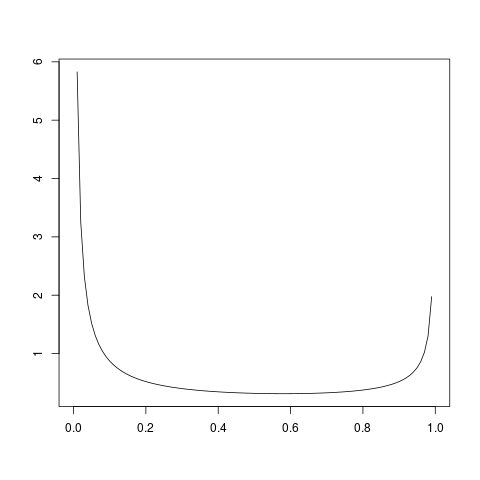
\includegraphics[scale=.5]{beta.png}
%     \label{fig:1}
%     \caption{The beta distribution maximizing $\biasratio$ (obtained numerically).}
% \end{figure}
  
  For $S$ exponentially distribution, $\biasratio = 1/2$. For a gamma
  distribution with shape parameter $a$,
  $\biasratio=\frac{16a}{a+1}(B(1/2,a,a+1)-1/2)^2$, where
  $B(1/2,k,k+1)=\int_0^{1/2}x^k(1-x)^{k+1}dx$ is an incomplete beta
  integral. Numerical evaluation suggests this expression is maximized
  at $k\approx .54$ with value $\approx .56$.

  
  When $S$ has a pareto distribution with shape parameter $a$, i.e., $f_S(s) =a\sigma^a/s^{a+1}\{s>\sigma\}$ when the scale parameter is $\sigma$,
  $$
  \biasratio = \frac{4a(a-2)}{((2a-1)(a-1))^2},
  $$
  defined for $a>2$ and maximized over $a$ at the unique root of $-2a^3+6a^2-2a-1$ on $(2,\infty)$,
  $$
  a=1+2\sqrt{2/3}\cos\left( 1/3\arctan\left(\sqrt{101/27}\right)  \right) \approx 2.53,
  $$
  where it takes the value $\approx .14$.

  In practice, one may attempt to estimate $\biasratio$ using the
  data. This approach may introduce bias of its own, particularly when
  using common ratio estimators in conjunction with  smaller
  meta-analyses. The performance of an example of this approach is presented in Section \ref{section:simulations}.

  
\section{Simulations}
\label{section:simulations}
  We consider the Types I and II error rates for the standard and 
  debiased versions of Begg's test. To carry out the debiased version
  of Begg's test, we used both the true asymptotic bias, which depends
  on knowing the distribution of $\s$, and an approximation based on the
  data. For the latter, given a sample of study precisions
  $s_1,\ldots,s_n$, $\biasratio=(\E|\s_1-\s_2|)^2/E(\s^2)$ was estimated
  by
    \begin{align}
      \left({n\choose 2}^{-1}\sum_{j<k}|s_j-s_k|\right)^2\bigg/ \overline{s^2}.
    \end{align}
    The scripts used to run the simulations and produce the figures in
    this section, as well as a supporting \texttt{R} package, are
    available at \url{https://github.com/haben-michael/begg-public}.

      \begin{enumerate}
      
  \item FPR control
    
    To examine the Type 1 error rate, data is generated under the null
    model (\ref{model:symmetric}). The distributions of $\s$
    considered were uniform, beta, exponential, gamma, and pareto,
    with the parameters given in Section
    \ref{section:theory:gaussian}. Three meta-analysis sample sizes
    were considered, 25, 75, and 150. The sizes 25 and 75 were chosen
    to match the sizes used in \citet{begg1994a}. The size 150 was
    chosen to illustrate the conclusion of Theorem \ref{theorem:1} that
    the bias in Begg's test persists with large sample sizes. The test
    was conducted at a nominal level of 5\%. There were 1000 monte
    carlo repetitions.

    The results are presented in Table \refeq{table:fpr}. The unadjusted
    Begg test is conservative and consistent with the discussion in
    Section \ref{section:theory:source of bias} this bias does not go away with increased
    sample size.  The magnitude of the asymptotic bias follows the
    order one expects from Table \ref{table:biasratio}: i.e., beta, gamma, uniform,
    pareto from most to least severe. For the small meta-analyses the
    corrected test exceeds the nominal level by 1--3\%, matching the
    nominal level for the larger meta-analysis. There does not appear
    to be much loss in approximating the correct variance using the
    data rather than using the true variance, even for the smaller
    meta-analysis.

    Next, we examine the Type 1 error rate under the normal
    random effects model, commonly used to model effect heterogeneity
    \citep{dersimonian1986}. Under this model, the variances of the
    study effects, denoted $\sigma^2$ in \eqref{model:nonpara}, are
    not the variances reported by study authors. Instead, the reported
    variances represent only the within-study variance, which is
    inflated by a between-study variance $\tau^2$ common to the
    studies to obtain the marginal variances of the study effects,
    i.e., $\y_j\sim
    \mathcal{N}(\mu,\sigma^2+\tau^2),j=1,\ldots,n$. Application of
    Theorem \ref{theorem:1}, which uses the marginal variance,
    therefore requires estimation of the between-study variance, for
    which we use a standard method of moments estimator
    \citep{dersimonian1986}.

    Table \refeq{table:fpr_hetero} presents
    the observed Type 1 error rates of the unadjusted Begg test using
    the true between-study variance, the adjusted Begg test also using
    the true between-study variance, and adjusted Begg test using the
    estimated between-study variance. The results are similar to those
    observed in Table \refeq{table:fpr}. Also presented for each
    within-study precision distribution is the average $I^2$, a
    standard measure of effect heterogeneity.

    
  \item Type II error rate

    % Examination of the Type 2
    % error rate requires the specification of a selection model. We f
    We examine the Type II error rate under an alternative considered
    by \citet{begg1994a}. Under this alternative, a study with p-value $p$
    is selected for publication with probability $\propto\exp(-bp)$,
    with $b\ge 0$. The parameter $b$ controls the strength of
    selection, with $b=0$ corresponding to no selection. The choice of
    selection function was informed by studies of selection bias
    contemporaneous with \citet{begg1994a}. The distributions of $\s$
    considered for this simulation were uniform, beta, exponential and gamma, and the sizes
    of the meta-analyses considered were 25, 75, and 150.

    Power curves are presented in Fig. \refeq{fig:power}. For
    ease of interpretation, the alternatives are parameterized by the
    proportion of studies selected, rather than $b$. The improvement
    in power across distributions and sizes has a median value of
    17\%.  The estimator based on the approximation to the true
    asymptotic variance performs similarly to the oracle estimator.% \comment{maybe show this by simulation.}
    
  \end{enumerate}
  
  % \item re-analysis of meta-analysis?

    \section{Data analysis}\label{section:data analysis}

    As an application, we describe three meta-analyses chosen to
    illustrate different conclusions drawn by the standard and
    bias-corrected Begg's test. In the typical situation that Begg's
    test reports a p-value far from the analyst's chosen threshold, the
    bias-corrected test will agree with the biased test. In the
    selected examples, the standard Begg's test reports p-values in the range
    $5-10\%$ and would be insignificant at the $5\%$ level. The three
    examples were chosen to contrast the stength of evidence for
    publication bias conveyed by a funnel plot, the conventional
    informal test for publication bias. In the first, the authors see
    little evidence for publication bias based on a funnel plot. In
    the second, the authors are unable to determine the risk of
    publication bias. In the third, the authors caution that studies
    have likely been omitted.
    
    % In the first, an informal analysis
    % suggests that publication bias may be present, and this conclusion
    % is contradicted by the standard Begg's test. In the second, an
    % informal analysis and the standard Begg's test conducted at the
    % $5\%$ level both offer little indication of publication bias.  For
    % both meta-analyses the bias bias-corrected Begg's test returns a
    % p-value $<2\%$. % Both meta-analyses were chosen with mean differences of
    % % continuous data as effects to make the gaussian assumption of
    % % Theorem \ref{theorem:1} more plausible.
    
    % In a 2014 analysis, \citet{zhang2014} assess the therapeutic effects of
    % Astragalus (\emph{Radix Astragali}), a traditional remedy, in
    % treating kidney disease. As part of their analysis, the authors
    % examine whether Astragalus is associated with a decrease in serum
    % creatinine, high levels of which are associated with poor kidney
    % health. To do so they conduct a meta-analysis of 13 randomized and
    % quasi-randomized trials together involving 775 subjects. The
    % conclusion of the meta-analysis is that Astragalus is associated
    % with a decrease of $‐21.39$ \textmu mol/L relative to control, with a
    % $95\%$ CI $(‐34.78, ‐8)$, and a p-value of $.17\%$. Upon
    % examining a funnel plot [see...], the authors warn of the
    % possibility of publication bias. On these data, however, the usual
    % Begg's test returns as p-value $5.5\%$, which just fails to give
    % significant evidence of publication bias at the $5\%$ level. On
    % the other hand, the bias-corrected Begg's test returns as p-value
    % $1.6\%$, confirming the authors' suspicions.

    In a 2005 analysis, \citet{van2005} assess the therapeutic effects
    of alpha-glucosidase inhibitors in treating type 2 diabetes
    mellitus. As part of this analysis, they examine the change in
    body weight under treatment. In a meta-analysis based on 13
    randomized trials of at least 12 weeks' duration together
    involving 864 subjects, the authors find little or no effect of
    the treatment on weight, contrary to expectations based on earlier
    work. The authors assess the likelihood of publication bias as low
    based on a funnel plot (Fig. \ref{fig:funnel}), and Begg's test
    gives a p-value of $7.4\%$ . The bias-corrected test, however,
    rejects at the $5\%$ level with a p-value of $2.7\%$. In this case
    the possibility of publication bias, suggested by the
    bias-corrected test, is arguably of less concern as the subsequent
    meta-analysis can't be a false positive, failing to be significant
    anyway.

    In a 2016 analysis, \citet{mcnicol2016} assess the therapeutic
    effects of intravenously administered paracetamol in treating
    postoperative pain. As part of their analysis, they examine the
    reduction in opioids administered under treatment by
    paracetamol. In a meta-analysis of 13 randomized trials together
    involving $777$ subjects, the authors find a highly significant
    reduction of $1.92$ mg, with a $95\%$ CI $(-2.41,-1.42)$. The
    authors assess the quality of the data as moderate, noting that
    the risk of selective reporting is unclear. In this case, a
    standard Begg's test gives a p-value $5.2\%$, just insignificant
    at the $5\%$ level, whereas the bias-corrected test returns a
    p-value $2.6\%$, suggesting publication bias is present and
    casting doubt on the validity of the significant result of the
    subsequent meta-analysis. A funnel plot (Fig. \ref{fig:funnel})
    likewise suggests the presence of publication bias.
    
    In a 2020 analysis, \citet{hooper2020} assess the effect of low-fat
    intake on body weight in populations not seeking to lose
    weight. The authors conduct a meta-analysis on 26 randomized
    trials of at least six months' duration involving $50,907$
    subjects. They find that a low-fat diet is associated with a
    $-1.56$ kg difference in weight, with a $95\%$ CI $(-1.88,-1.23)$,
    and a p-value reported as $<.00001$. Though the trials in this
    analysis were chosen in part for their low risk of bias,
    the authors warn of the possibility of selection bias based on a
    funnel plot (Fig. \ref{fig:funnel}) and other analyses. Begg's test, however, gives a
    p-value $7.8\%$, whereas the corrected test gives a p-value
    $3.3\%$, consistent with the authors' suspicions.

    
    
\section{Conclusion}

  We have examined the causes of a known bias in Begg's test and
  quantified it in the common model of normally distributed
  studies. We have also suggested a debiased estimator that matches
  the nominal variance in the limit as the number of studies grows,
  unlike the standard estimator, which remains conservative. Although
  simulations suggest the corrected estimator is somewhat anticonservative on
  smaller meta-analyses, from the perspective of an analyst
  concerned primarily about the integrity of the meta-analysis,
  exceeding the nominal level may be preferable to falling under it,
  as discussed earlier.  % \comment{maybe mention the poor performance of beggs test}

  Various avenues of further research suggest themselves. First, the
  direction of the bias of Begg's test outside of the gaussian model,
  characterized by (\ref{eqn:iff_cond}) for symmetric distributions,
  has not been fully explored here. It is possible that the direction
  is the same for certain common large classes, e.g., symmetric unimodal
  distributions. % Second, even in the gaussian model, the magnitude of
  % the bias given by $\frac{(\E|\s_1-\s_2|)^2}{\pi\E(\s^2)}$
  % has only here been studied in relation to a few select distributions
  % for the study variance. For example, a distribution maximizing this
  % quantity has not been produced. 
  Second, a glance at
  Fig. \ref{fig:power} shows that, even with the boost in power
  provided by the debiased estimator, the power curves of Begg's test
  are not very reassuring. There are competitors to Begg's test, such
  as Egger's test and the more recent test of \citet{lin2018}. However, 
  quantitative conditions have not been provided to assist an analyst
  in deciding which test to prefer in given situations.

\begin{figure}
  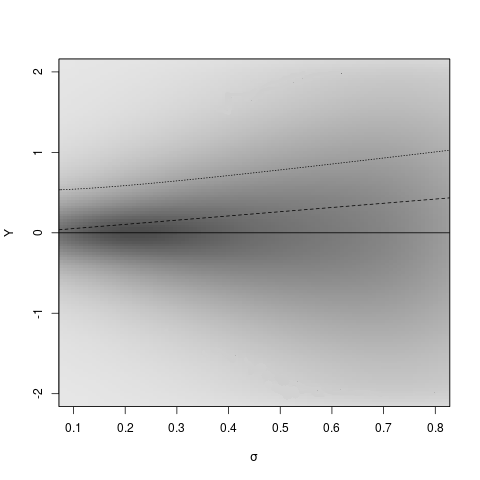
\includegraphics[width=\linewidth]{selection.png}
  \caption{  The effect of a simple hard thresholding selection model on the
  study means. Overlaid on the joint density of $\y$ and $\sigma$, indicated by grayscale, is the mean $\theta=0$ of $\y|\sigma$
  before selection and exhibiting no
  trend (solid line), a threshold line corresponding to rejecting studies with a one-sided p-value
  $>.3$ (dashed line), and the mean of the studies
  after selection, exhibiting a trend that Begg's test can pick up (dotted line).
}
  \label{fig:selection}
\end{figure}
  
% \item possible additions: lower power curve? proposed solution[done]? nonnormal response? asymptotic normality
% \end{enumerate}
  % [give table of distributions of common nonnegative rv's with common values for $\biasratio$ and the resulting bias]

% \begin{figure}
%   \centering
%   \begin{subfigure}{.5\textwidth}
%     \centering
%     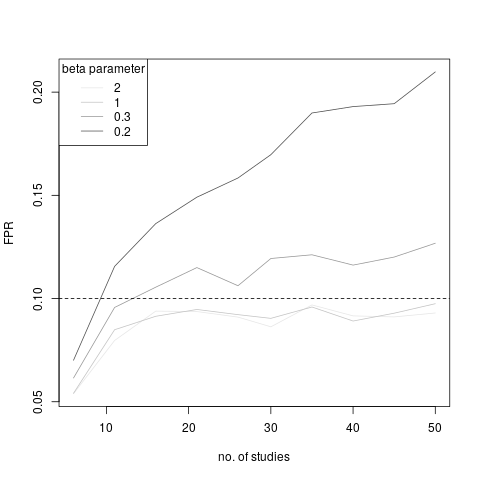
\includegraphics[width=\linewidth]{neg_bias_beta}
%     % \caption{A subfigure}
%     % \label{fig:sub1}
%   \end{subfigure}%
%   \begin{subfigure}{.5\textwidth}
%     \centering
%     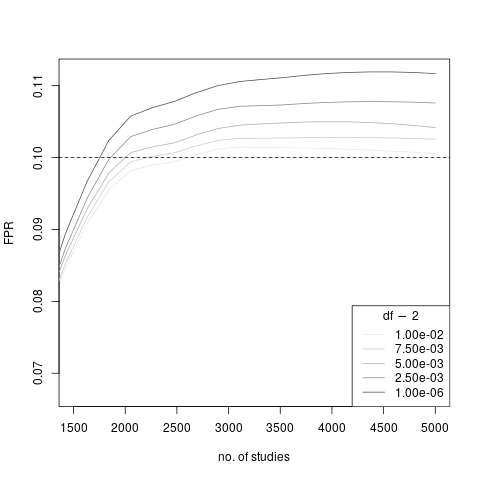
\includegraphics[width=\linewidth]{neg_bias_students}
%     % \caption{A subfigure}
%     % \label{fig:sub2}
%   \end{subfigure}
%   \caption{The average Type I error rate of Begg's test when the
%     response distribution is based on (left) a centered, symmetric beta
%     distribution and (right) Student's t distribution. The error
%     control is lost with (left) bimodality or (right) fewer degrees of
%     freedom. Both situations are arguably pathological in the context
%     of a meta-analysis and unlikely to be encountered in practice. The
%     precision distribution for the studies was simlated as uniform on
%     $[1,4]$.}
%   \label{fig:negative bias}
%   \end{figure}

% \begin{figure}
%   \includegraphics[width=\linewidth]{students.png}
%   \caption{The average Type I error rate of Begg's test when the
%     response distribution is based on (left) a shifted beta
%     distribution and (right) Student's t distribution. The error
%     control is lost with (left) bimodality or (right) fewer degrees of
%     freedom. Both situations are arguably pathological in the context
%     of a meta-analysis and unlikely to be encountered in practice. The
%     precision distribution for the studies was simlated as uniform on
%     $[1,4]$.}
%   \label{fig:negative bias}
% \end{figure}

\begin{figure}
  \centering
  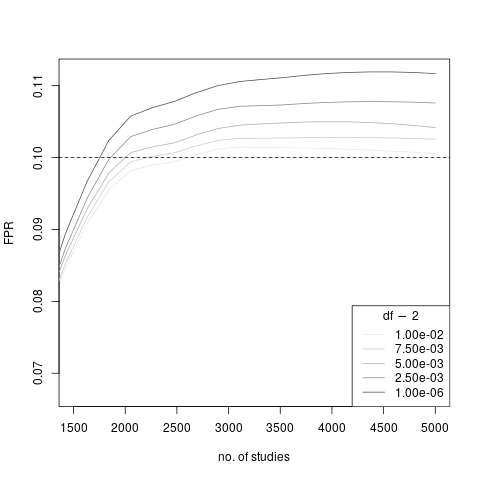
\includegraphics[width=\linewidth/2]{neg_bias_students.png}
  \caption{The observed Type I error rate of Begg's test compared to a
    nominal rate of .1 when the distribution of the response $Z$ is
    based on a standardized Student's t distribution, i.e.,
    $Z=T/\sqrt{df/(df-2)}$ where $T$ follows a Student's t with $df$
    degrees of freedom. The error rate slightly exceeds the nominal
    rate, particularly as $df$ decreases to the boundary case at
    $2$. In contrast, when $Z$ is gaussian, the error rate falls below
    the nominal rate.}
  \label{fig:negative bias}
\end{figure}

\begin{table}
    \begin{tabular}{l c c}
    distribution of $S$ & $\biasratio$ & max asymptotic bias \\
    \hline\\
    uniform  & $\frac{(b-a)^2}{3(a^2+b^2+ab)}$  & .11\\
    beta & $\left(\frac{4B(a+b,a+b)}{B(a,a)B(b+b)}\right)^2\frac{a+b+1}{a(a^2+ab+a+b)}$ & .21\\
    % exponential & 1/2 & .16\\
    gamma & $\frac{16a}{a+1}(B(1/2,a,a+1)-1/2)^2$ & .18\\
    pareto & $\frac{4a(a-2)}{((2a-1)(a-1))^2}$ & .04\\
  \end{tabular}
  \caption{Shape families of some nonnegative RVs,
    $\biasratio=\text{bias}\times\pi=(\E|S_1-S_2|)^2/E(S^2)$ in terms
    of the shape parameters, and the maximum bias of the asymptotic
    variance over the shape family. The maximum variance was obtained
    numerically for the beta and gamma distributions.}
  \label{table:biasratio}
\end{table}

\begin{table}
  % latex table generated in R 4.1.0 by xtable 1.8-4 package
% Sat Jan 29 00:43:38 2022
\begin{tabular}{rlll}
  \hline
  & \multicolumn{3}{c}{meta-analysis size} \\
 precision distribution &25&75&150\\
 \hline
uniform & 0.04, 0.07, 0.07 & 0.03, 0.05, 0.05 & 0.03, 0.05, 0.05 \\ 
  exponential & 0.03, 0.08, 0.08 & 0.02, 0.06, 0.06 & 0.02, 0.05, 0.05 \\ 
  gamma & 0.02, 0.07, 0.07 & 0.02, 0.06, 0.06 & 0.01, 0.05, 0.05 \\ 
  beta & 0.01, 0.08, 0.07 & 0.01, 0.06, 0.05 & 0.01, 0.05, 0.05 \\ 
  pareto & 0.05, 0.06, 0.06 & 0.04, 0.06, 0.06 & 0.04, 0.05, 0.05 \\ 
   \hline
\end{tabular}

  \caption{False positive rates for the standard Begg's test, after debiasing using the true asymptotic bias, and after debiasing using an estimate of the asymptotic bias.}
  \label{table:fpr}
\end{table}

\begin{table}
  % latex table generated in R 4.1.0 by xtable 1.8-4 package
% Fri Feb  4 21:26:30 2022
\begin{tabular}{rlll}
  \hline
  & \multicolumn{3}{c}{meta-analysis size} \\
 precision distribution &25&75&150\\
 \hline
uniform $(I^2=0.54)$ & 0.05, 0.07, 0.07 & 0.03, 0.05, 0.05 & 0.03, 0.05, 0.05 \\ 
  exponential $(I^2=0.85)$ & 0.05, 0.07, 0.07 & 0.04, 0.06, 0.06 & 0.04, 0.05, 0.05 \\ 
  gamma $(I^2=0.67)$ & 0.03, 0.06, 0.06 & 0.02, 0.06, 0.06 & 0.02, 0.05, 0.05 \\ 
  beta $(I^2=0.39)$ & 0.01, 0.07, 0.07 & 0.01, 0.05, 0.05 & 0.01, 0.06, 0.06 \\ 
  pareto $(I^2=0.92)$ & 0.06, 0.06, 0.06 & 0.06, 0.06, 0.06 & 0.06, 0.06, 0.06 \\ 
   \hline
\end{tabular}

  \caption{False positive rates under effect heterogeneity for the standard Begg's test using the true (unobserved) between-study variance, after debiasing using an estimate of the asymptotic bias while still using the true (unobserved) between-study variance, and after debiasing using an estimate of the asymptotic bias and an estimate of the between-study variance.}
  \label{table:fpr_hetero}
\end{table}

% \begin{figure}
  %   \centering
  %   \resizebox{250pt}{!}{%
  %     % latex table generated in R 4.1.0 by xtable 1.8-4 package
% Sat Jan 29 00:43:38 2022
\begin{tabular}{rlll}
  \hline
  & \multicolumn{3}{c}{meta-analysis size} \\
 precision distribution &25&75&150\\
 \hline
uniform & 0.04, 0.07, 0.07 & 0.03, 0.05, 0.05 & 0.03, 0.05, 0.05 \\ 
  exponential & 0.03, 0.08, 0.08 & 0.02, 0.06, 0.06 & 0.02, 0.05, 0.05 \\ 
  gamma & 0.02, 0.07, 0.07 & 0.02, 0.06, 0.06 & 0.01, 0.05, 0.05 \\ 
  beta & 0.01, 0.08, 0.07 & 0.01, 0.06, 0.05 & 0.01, 0.05, 0.05 \\ 
  pareto & 0.05, 0.06, 0.06 & 0.04, 0.06, 0.06 & 0.04, 0.05, 0.05 \\ 
   \hline
\end{tabular}

  %   }
  %   \captionof{figure}{Causal DAG describing longitudinal confounding with $T=2$ time points.}
  %   \label{fig:sra dag}
  % \end{figure}

\begin{figure}
  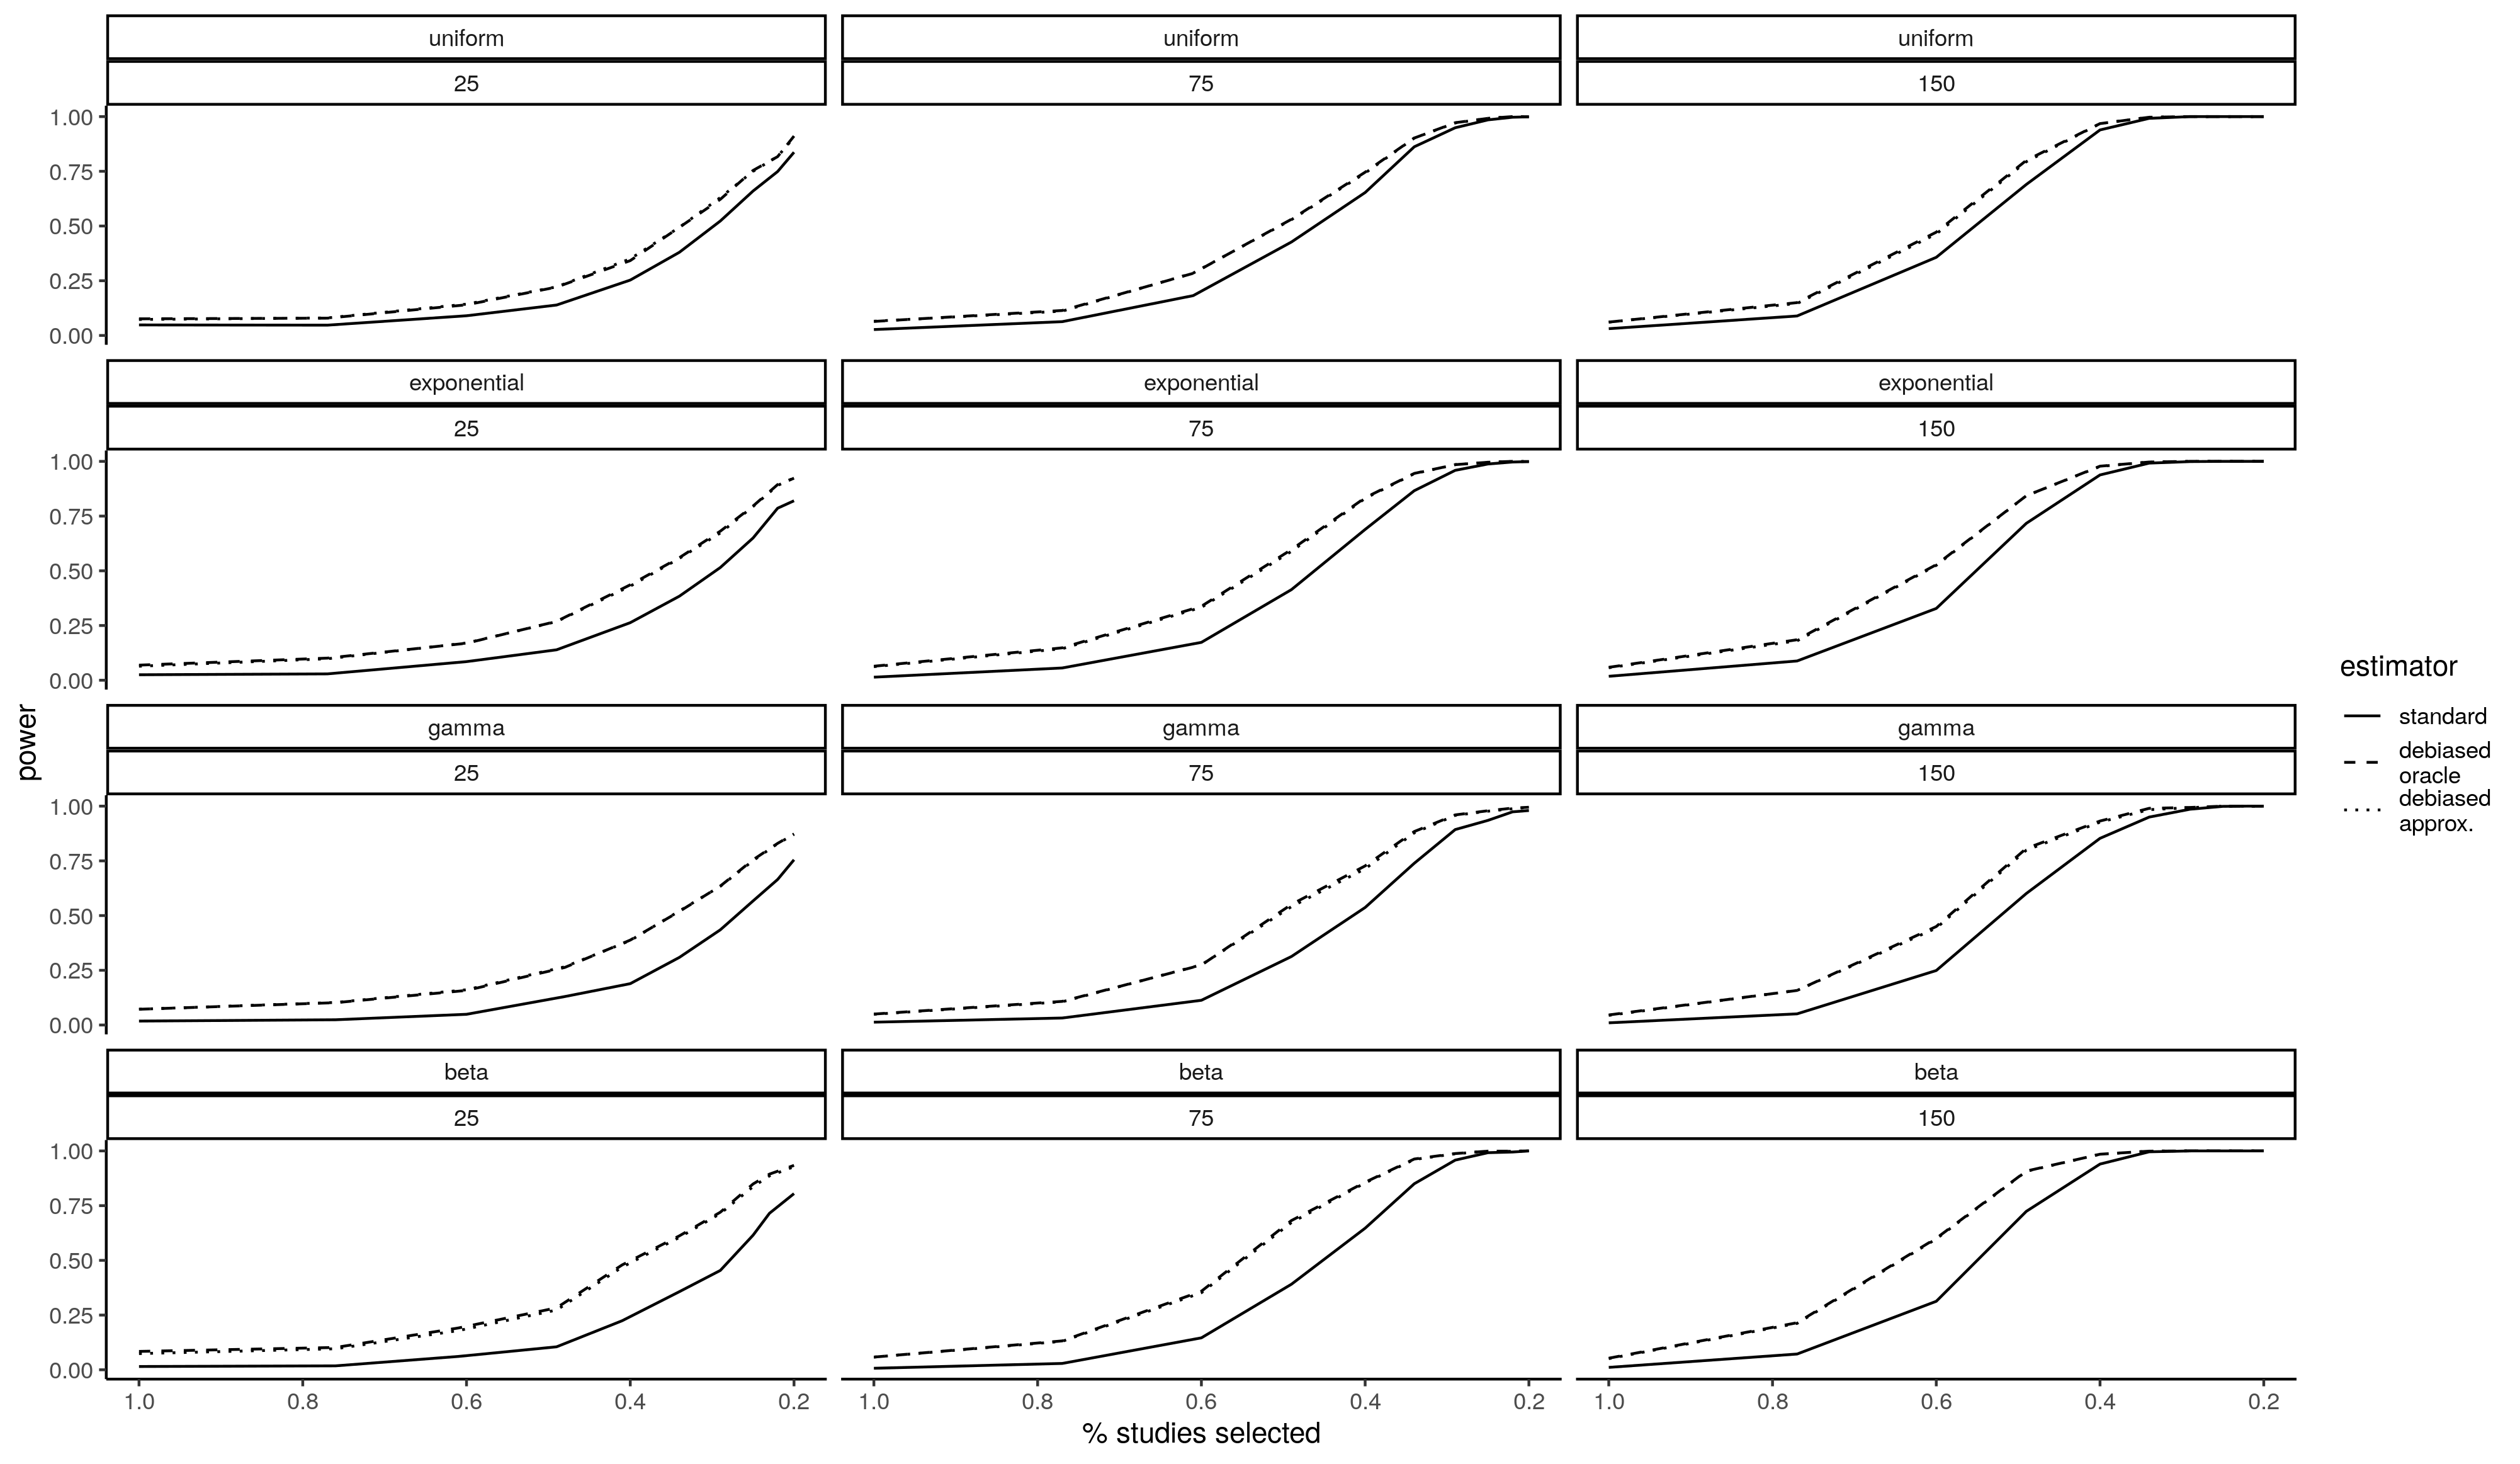
\includegraphics[width=\linewidth]{power_curves.png}
  % 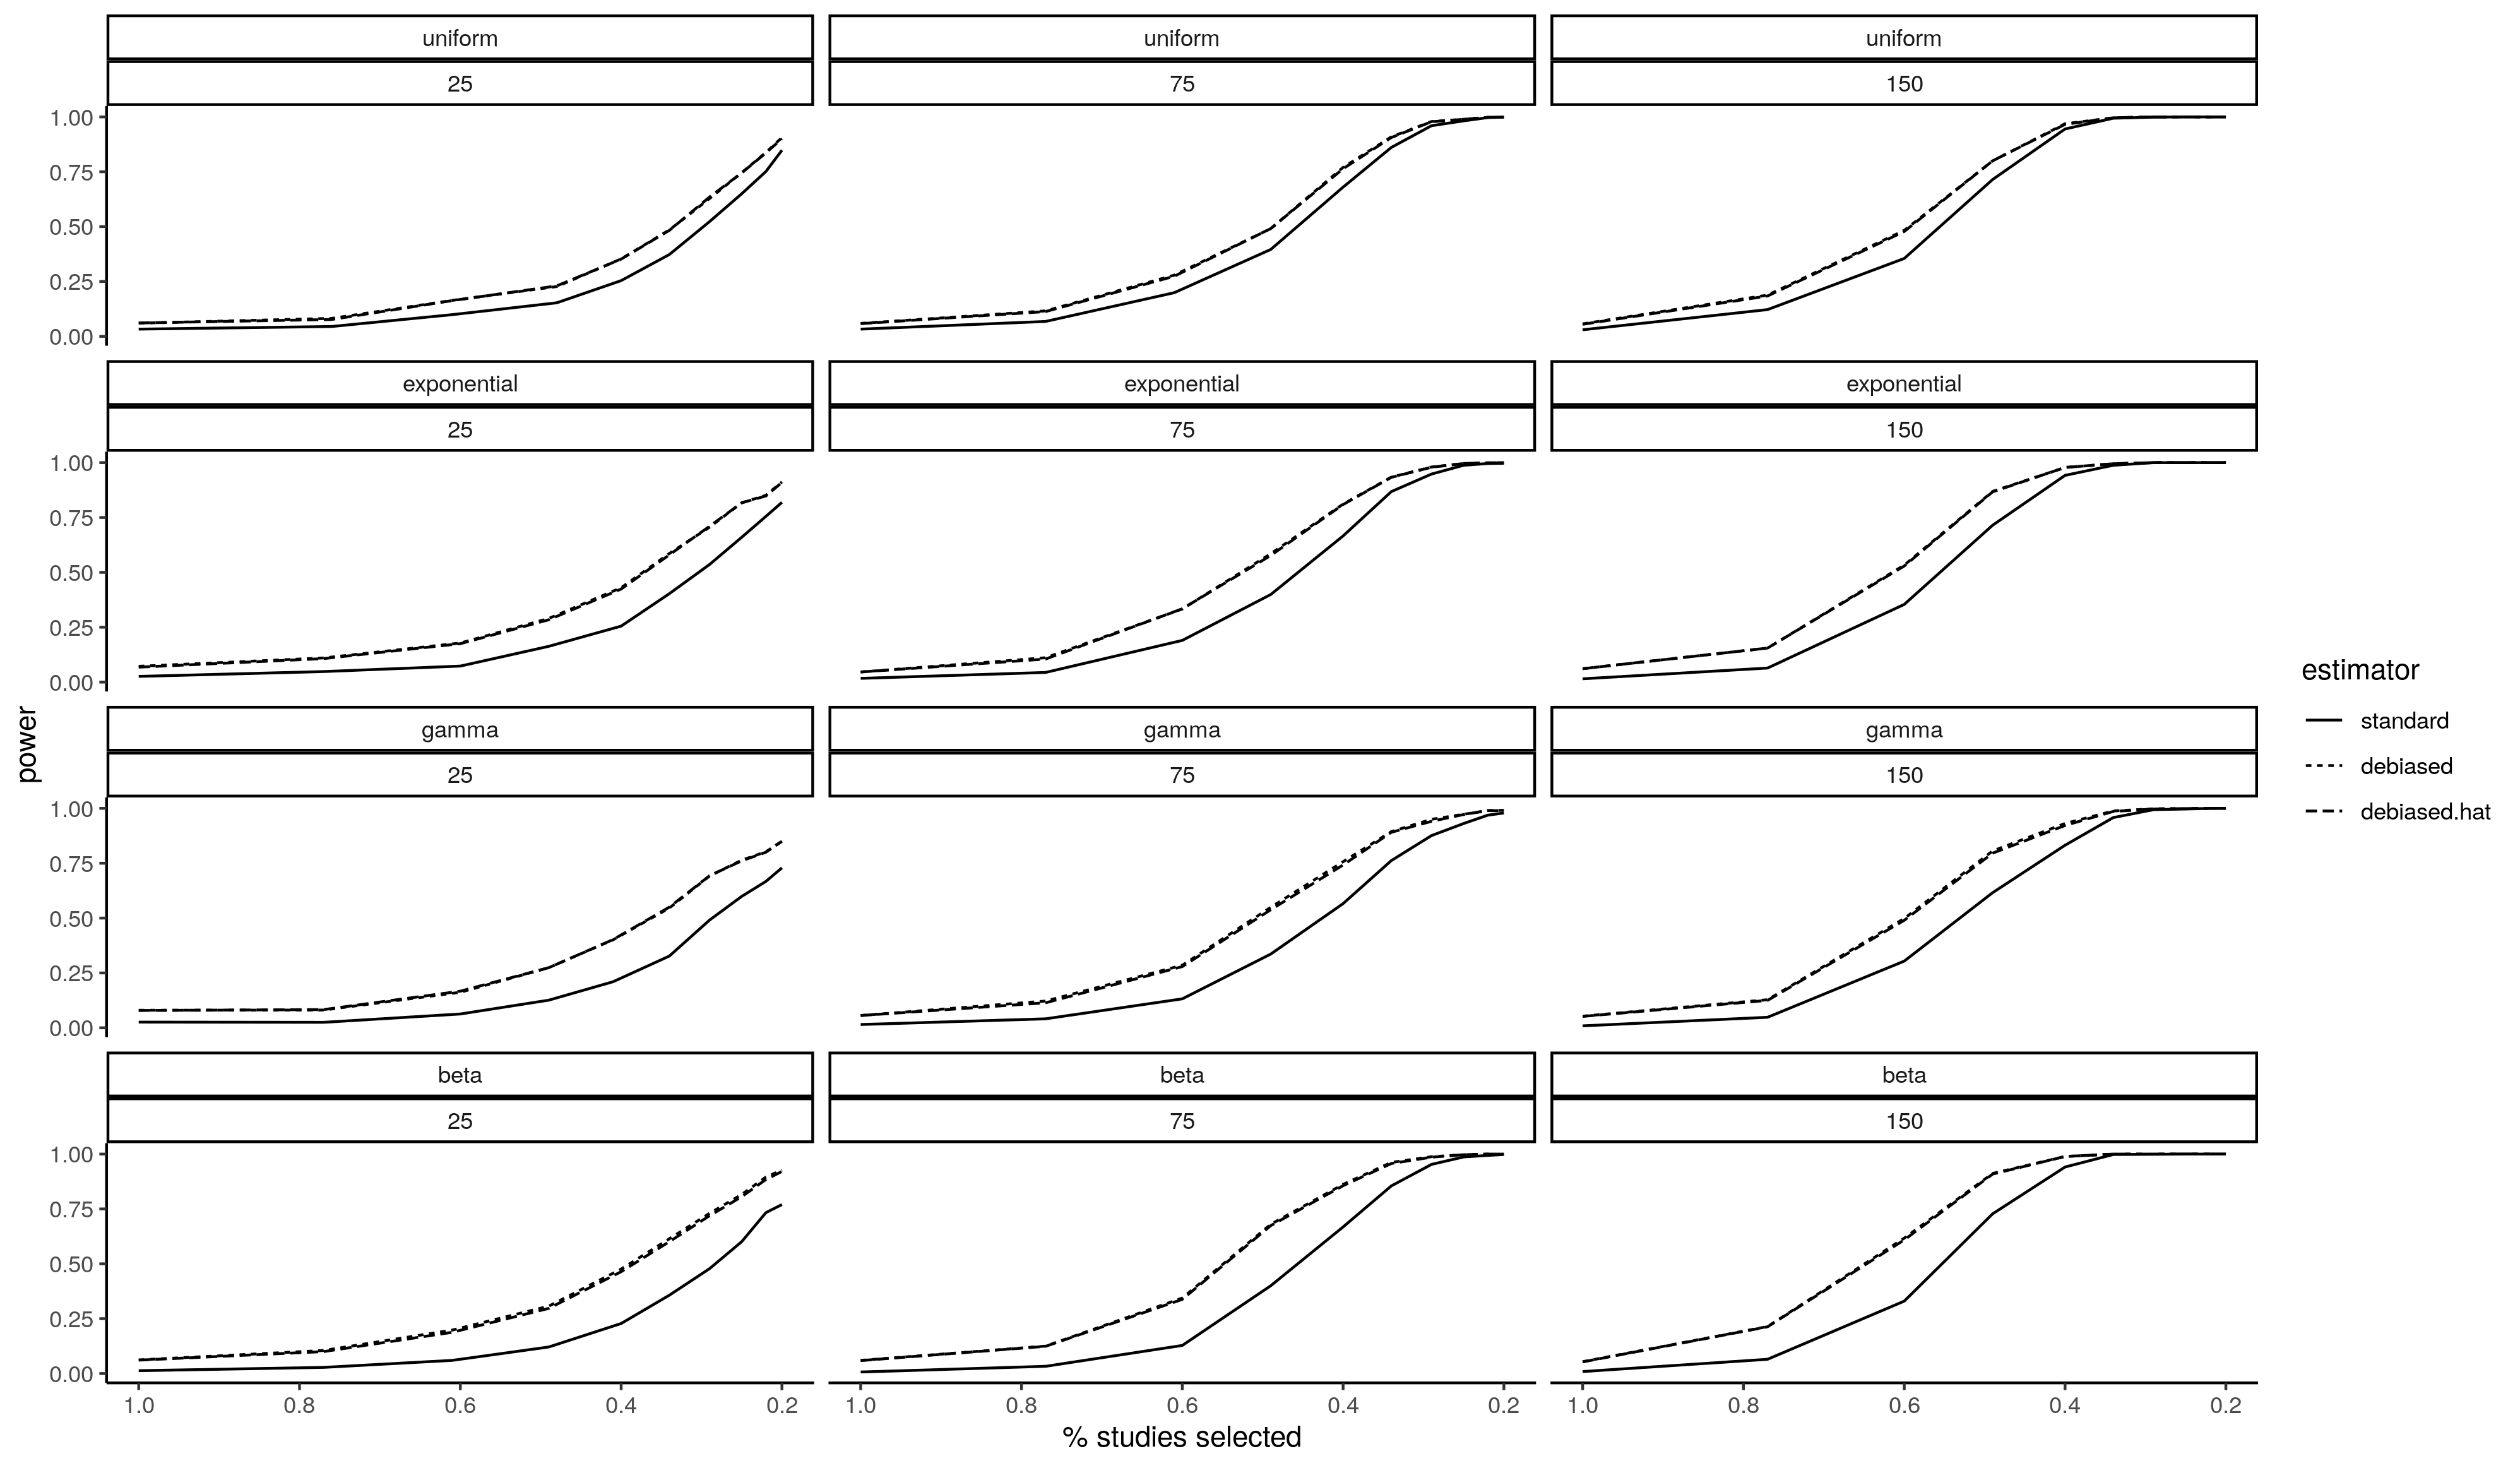
\includegraphics[scale=.5]{ms/210314a.png}
  \caption{Power curves of standard Begg's test, after debiasing using true asymptotic bias, and after debiasing using estimated asymptotic bias. The alternatives are parameterized by the proportion of studies selected. The estimator debiased using an estimate of the true bias and the true bias itself overlap.\comment{increase size of plot}}
  \label{fig:power}
\end{figure}

\begin{figure}
  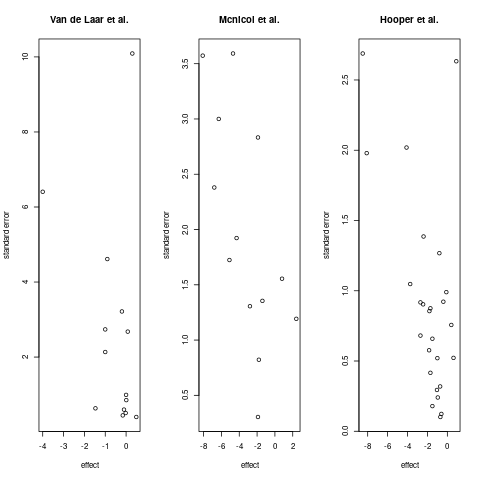
\includegraphics[width=\linewidth]{funnel_plots.png}
  \caption{Funnel plots of the three meta-analyses described in Section \ref{section:data analysis}. These were interpreted as suggesting lower, moderate, and higher possibilities of publication bias, going from left to right.}
  \label{fig:funnel}
\end{figure}


% \bibliographystyle{plain}
% \bibliographystyle{plainnat}
\bibliographystyle{chicago}
\bibliography{begg.bib}
% \begin{thebibliography}{7}
%   \providecommand{\natexlab}[1]{#1}
%   \providecommand{\url}[1]{\texttt{#1}}
%   \expandafter\ifx\csname urlstyle\endcsname\relax
%   \providecommand{\doi}[1]{doi: #1}\else
%   \providecommand{\doi}{doi: \begingroup \urlstyle{rm}\Url}\fi

% \bibitem[Begg(1994)]{begg1994b}
%   Colin Begg.
%   \newblock Publication bias.
%   \newblock In Harries Cooper and Larry Hedges, editors, \emph{The Handbook of
%     Research Synthesis}, pages 399--409. Russel Sage Foundation, New York, 1994.

% \bibitem[Begg and Mazumdar(1994)]{begg1994a}
%   Colin Begg and Madhuchhanda Mazumdar.
%   \newblock Operating characteristics of a rank correlation test for publication
%   bias.
%   \newblock \emph{Biometrics}, pages 1088--1101, 1994.

% \bibitem[Gjerdevik and Heuch(2014)]{gjerdevik2014}
%   Miriam Gjerdevik and Ivar Heuch.
%   \newblock Improving the error rates of the begg and mazumdar test for
%   publication bias in fixed effects meta-analysis.
%   \newblock \emph{BMC Medical Research Methodology}, 14\penalty0 (1):\penalty0
%   1--16, 2014.

% \bibitem[Van~de Laar et~al.(2005)Van~de Laar, Lucassen, Akkermans, Van~de
%   Lisdonk, Rutten, and Van~Weel]{van2005}
%   Floris~A Van~de Laar, Peter~LBJ Lucassen, Reinier~P Akkermans, Eloy~H Van~de
%   Lisdonk, Guy~EHM Rutten, and Chris Van~Weel.
%   \newblock Alpha-glucosidase inhibitors for type 2 diabetes mellitus.
%   \newblock \emph{Cochrane database of systematic reviews}, \penalty0 (2), 2005.

% \bibitem[McNicol et~al.(2016)McNicol, Ferguson, Haroutounian, Carr, and
%   Schumann]{mcnicol2016}
%   Ewan~D McNicol, McKenzie~C Ferguson, Simon Haroutounian, Daniel~B Carr, and
%   Roman Schumann.
%   \newblock Single dose intravenous paracetamol or intravenous propacetamol for
%   postoperative pain.
%   \newblock \emph{Cochrane database of systematic reviews}, \penalty0 (5), 2016.


% \bibitem[Lin and Chu(2018)]{lin2018}
%   Lifeng Lin and Haitao Chu.
%   \newblock Quantifying publication bias in meta-analysis.
%   \newblock \emph{Biometrics}, 74\penalty0 (3):\penalty0 785--794, 2018.

% \end{thebibliography}



% \begin{appendices}
\section*{Appendix}
% \stepcounter{section}
\label{appendix:proof}
  % \renewcommand\thechapter{}
  % \renewcommand\thesection{\arabic{section}}
  % \renewcommand\thesubsection{\thesection.\arabic{subsection}}
  % \renewcommand\thefigure{\arabic{figure}}
  % \renewcommand\thetable{\arabic{table}}
  % \chapter{}
  
  
% old marginal theorem proof
% \begin{proof}[Proof of Theorem \ref{theorem:1}]
%    As discussed above, any bias in the asymptotic variance relative to 4/9 is due to the term %(\refeq{eqn:cov_bias_source})
%     \begin{align}
%       % \Cov_{1234} = \P(\frac{z_1-z_2}{s_1-s_2}\wedge \frac{z_3-z_4}{s_3-s_4}>\hat{\theta}) - \P(\frac{z_1-z_2}{s_1-s_2} > \hat{\theta})^2
%       \P\left(\frac{\z_1-\z_2}{\s_1-\s_2}\wedge \frac{\z_3-\z_4}{\s_3-\s_4}>\thetahat\right) - 1/4.
%       \label{thm1:cov_bias_source}
%     \end{align}
%     % By the symmetry of $z_j$, $\P(\frac{z_1-z_2}{s_1-s_2} > \hat{\theta})=1/2$.
%     The theorem follows on showing that % \comment{should be negative, also should have abs value sings to match theorem statement}
%     \begin{align}
%       % n\cdot \left(\P\left(\frac{z_1-z_2}{s_1-s_2}\wedge \frac{z_3-z_4}{s_3-s_4}>\hat{\theta}\mid s_1,\ldots,s_n\right)-\frac{1}{4}\right) \to \frac{(s_1-s_2)(s_3-s_4)}{4\pi\E(S^2)}
%       \P\left(\frac{\z_1-\z_2}{\s_1-\s_2}\wedge \frac{\z_3-\z_4}{\s_3-\s_4}>\thetahat\mid \s_1,\ldots,\s_n\right)-\frac{1}{4}
%       = -\frac{|\s_1-\s_2||\s_3-\s_4|}{4\pi\sum_{j=5}^n \s_j^2} + o(1/\sum_{j=5}^n \s_j^2)
%     \end{align}
%     and that $n$ times the right-hand side is uniformly integrable, since then the LLN gives
%     \begin{align}
%       \begin{split}
%       \V(\sqrt{n}\tau) - 4/9 &= 4n \cdot (Eq.\hspace{.05in} \eqref{thm1:cov_bias_source}) + o(1)\\
%                                &= 4n\E\left( -\frac{|\s_1-\s_2||\s_3-\s_4|}{4\pi\sum_{j=5}^n \s_j^2} + o(1/\sum_{j=1}^n \s_j^2) \right) + o(1)\\
%                                &\to -\E\left(\frac{(\E|\s_1-\s_2|)^2}{\pi\E(\s^2)}\right).
%                              \end{split}\label{thm1:conclusion}
%     \end{align}
    
%     Since $\z_1,\ldots\z_n,$ are independent of $\s_1,\ldots,\s_n$, the probability in (\refeq{thm1:cov_bias_source}) is
%     \begin{align}
%       &\P\left(\frac{\sum_{j=5}^n \z_j\s_j}{\sum_j \s_j^2} < \left(\frac{\z_1-\z_2}{\s_1-\s_2}- \frac{\sum_{j=1}^4\z_j\s_j}{\sum_j\s_j^2}  \right)\wedge \left(\frac{\z_3-\z_4}{\s_3-\s_4}- \frac{\sum_{j=1}^4\z_j\s_j}{\sum_j\s_j^2}\right) \bigg\vert \svec_n\right)\\
%       &=\E\left(\Phi\left(\frac{\sum_j\s_j^2}{\sqrt{\sum_{j=5}^n\s_j^2}}\left(\frac{\z_1-\z_2}{\s_1-\s_2}- \frac{\sum_{j=1}^4\z_j\s_j}{\sum_j\s_j^2}  \right)\wedge \left(\frac{\z_3-\z_4}{\s_3-\s_4}- \frac{\sum_{j=1}^4\z_j\s_j}{\sum_j\s_j^2}\right)  \right) \bigg\vert \svec_n\right)\\
%       &=\E\left(\Phi(\w_0\wedge \w_1)\mid \svec_n\right),\label{thm1:min_exp}
%     \end{align}
%     where $\w_0,\w_1$ are jointly normal conditionally on $\vec{\s}_n=(\s_1,\ldots,\s_n)$ with mean $0$, variances
%     $$
%     V_0=\frac{2}{(\s_1-\s_2)^2} + \frac{2}{\sum_j\s_j^2}+\frac{\sum_{1}^4\s^2}{(\sum_j\s_j^2)^2}, \hspace{10px}    V_1=\frac{2}{(\s_3-\s_4)^2} + \frac{2}{\sum_j\s_j^2}+\frac{\sum_{1}^4\s^2}{(\sum_j\s_j^2)^2},
%     $$
%     and covariance
%     $$
%     \rho\sqrt{V_0V_1}=-\frac{2}{\sum_j\s_j^2}+\frac{\sum_{1}^4\s^2}{(\sum_j\s_j^2)^2}.
%     $$
%     The density $f_{\w_0\wedge \w_1}$ of the minimum of a bivariate normal pair is readily available and substitution into (\refeq{thm1:min_exp}) gives
%     \begin{align}
%       &\E\left(\Phi(\w_0\wedge \w_1)\mid \vec{\s}_n\right) = \int_{-\infty}^{\infty}\Phi(u)f_{\w_0\wedge \w_1}(u)du\\
%       &=\sum_{j\in\{0,1\}}\frac{1}{\sqrt{V_j}}\int_{-\infty}^{\infty}\Phi(u)\Phi\left(\frac{u}{\sqrt{1-\rho^2}}\left(\frac{\rho}{\sqrt{V_j}}-\frac{1}{\sqrt{V_{1-j}}}\right) \right)\phi\left(\frac{u}{\sqrt{V_j}}\right)du.
%     \end{align}
%     The integral inside the sum has the form
%     \begin{align}
%       \int_{-\infty}^{\infty}\Phi(\alpha_j u)\Phi(\beta_j u)\phi(\gamma_j u)du
%     \end{align}
%     with $\alpha_j=1,\beta_j=\frac{1}{\sqrt{1-\rho^2}}\left(\frac{\rho}{\sqrt{V_j}}-\frac{1}{\sqrt{V_{1-j}}}\right),$ and $\gamma_j = \frac{1}{\sqrt{V_j}}$. This integral may be computed by differentiating first with respect to $\alpha$ and then $\beta$ to put it in terms of elementary functions,
%     \begin{align}
%       \int_{-\infty}^\infty u^2\phi(\alpha_j u)\phi(\beta_j u)\phi(\gamma_j u)du=\frac{1}{2\pi(\alpha_j^2+\beta_j^2+\gamma_j^2)^{3/2}},
%     \end{align}
%     then integrating  twice to obtain $\frac{1}{2\pi\gamma_j}\arctan\left(\frac{\alpha_j\beta_j}{\gamma_j\sqrt{\alpha_j^2+\beta_j^2+\gamma_j^2}}\right)$ as the required definite integral up to a constant. The constant may be determined by taking limits as $1/(4\gamma_j)$, giving
%     \begin{align}
%       \E\left(\Phi(\w_0\wedge \w_1)\mid \vec{\s}_n\right) =\frac{1}{2}+\frac{1}{2\pi}\sum_j\arctan\left(\frac{\alpha_j\beta_j}{\gamma_j\sqrt{\alpha_j^2+\beta_j^2+\gamma_j^2}}\right).     
%     \end{align}

%     Let $\Delta_0=\s_1-\s_2$ and $\Delta_1=\s_3-\s_4$. After simplification, the last expression is
%     \begin{align}
%       \frac{1}{2}+\frac{1}{2\pi}\sum_j\arctan\left(-\frac{1}{\Delta_j^2}\left(\frac{1}{\Delta_0^2\Delta_1^2}-\left(\frac{1}{\Delta_0^2}+\frac{1}{\Delta_1^2}\right)\frac{1}{2\sum_j\s_j^2}\right)^{-1/2}\right).
%     \end{align}
%     Let $u=1/\sum_{j=5}^n\s_j^2$, so by the LLN $u\to 0$ almost surely. When $u=0$, the last expression is $1/2 + (2\pi)^{-1}\sum_j \arctan\left(-|\frac{\Delta_{1-j}}{\Delta_j}|\right)=1/4$. Expanding about $u=0$ and simplifying, 
%     \begin{align}
%       % \E\left(\Phi(\w_0\wedge \w_1)\mid \vec{\s}_n\right) &=\frac{1}{4} + \frac{u}{2\pi}\sum_j\frac{\partial}{\partial u}\arctan\left(-\frac{1}{\Delta_j^2}\left(\frac{1}{\Delta_0^2\Delta_1^2}+\left(\frac{1}{\Delta_0^2}+\frac{1}{\Delta_1^2}\right)\frac{1}{2\sum_j\s_j^2}\right)^{-1/2}\right)\bigg|_{u=0} + o(u)\\
%       \E\left(\Phi(\w_0\wedge \w_1)\mid \vec{\s}_n\right) &=\frac{1}{4} + \frac{u}{2\pi}\sum_j\frac{\mathrm{d}}{\mathrm{d} u}\arctan\left(-\frac{1}{\Delta_j^2}\left(\frac{1}{\Delta_0^2\Delta_1^2}-\left(\frac{1}{\Delta_0^2}+\frac{1}{\Delta_1^2}\right)\frac{u}{2}\right)^{-1/2}\right)\bigg|_{u=0} + o(u)\\
%       &=\frac{1}{4}-\frac{u}{4\pi}|\Delta_0\Delta_1| + o(u).
%     \end{align}
%     % By another application of the LLN, $n\cdot u \to 1/\E(S^2)$ and $n\cdot o(u)\to 0$ a.s.
%     % The sequence $n\cdot u=n/\sum_{j=5}^n \s_j^2, n=1,2,\ldots,$ consists of the harmonic means of the variances $\sigma^2_j$, upper bounded by the arithmetic means, known to form a uniformly integrable sequence under the assumption of integrability of $\sigma^2$. \comment{handle remainder term}
%     Passing the limit into the expectation in \refeq{thm1:conclusion} follows from the
%     eventual uniform integrability of the sequence
%     $n\cdot u=n/\sum_{j=5}^n \s_j^2, n=1,2,\ldots,$ which in turn follows from Lemma    \ref{lemma:1}.
    
    
%       \end{proof}


%   \begin{lemma}\label{lemma:1}
%     If $\x_1,\x_2,\ldots$ are nonnegative and IID, then the sequence
%     of reciprocals of the sample means
%     $n/(\sum_{j=1}^n\x_j),n=n_0,n_0+1,\ldots,$ is uniformly integrable
%     for some $n_0$ if and only if the common CDF of the $\x_j$ is
%     $O(x^\epsilon)$ for some $\epsilon>0$.
%   \end{lemma}

%   \begin{proof}
%     First, $n/(\sum_{j=1}^n\x_j)$ has moments $>1$, say $1+\epsilon$, for $n$ large enough. As $\P(\frac{1}{n}\sum_{j=1}^n\x_j<x)\le \P(\x_1<nx)^n$,
%     \begin{align}
%       \E\left(\left(\frac{n}{\sum_{j=1}^n\x_j}\right)^{1+\epsilon}\right) &=
%                                                       (1+\epsilon)\int_0^\infty x^\epsilon\P\left(\frac{n}{\sum_{j=1}^n\x_j}>x\right)dx\\
%                                                     &\le(1+\epsilon)\left(1+\int_1^\infty x^\epsilon\P\left(\sum_{j=1}^n\x_j<\frac{n}{x}\right)dx\right)\\
%                                                     &\lesssim (1+\epsilon)\left(1+\int_1^\infty x^\epsilon\left(\frac{n}{x}\right)^{n\epsilon}dx\right),
%     \end{align}
%     which is finite for $n > 1/\epsilon-1$.
%     Next, for such $n$,  the sample means $\frac{1}{n}\sum_{j=1}^n\x_j,n=1,2,\ldots,$ are a reverse martingale with respect to $\mathcal{F}_n=\sigma\{\sum_{j=1}^n\x_j,\sum_{j=1}^{n+1}\x_j,\ldots\}$. The conditional form of Jensen's inequality applied to the convex function $x\mapsto x^{-(1+\epsilon)}$ on $\mathbb{R}^+$ gives, for $k\in\mathbb{N}$,
%     \begin{align}
%       \E\left(\left(\frac{n+k}{\sum_{j=1}^{n+k}\x_j}\right)^{1+\epsilon}\right) &= \E\left(\left(\E\left(\frac{1}{n}\sum_{j=1}^n\x_j\bigg\vert\mathcal{F}_{n+k}\right)\right)^{-(1+\epsilon)}\right)\\
%                                                                                 &\le \E\left(\left(\frac{1}{n}\sum_{j=1}^n\x_j\right)^{-(1+\epsilon)}\right) =
%                                                                                   \E\left(\left(\frac{n}{\sum_{j=1}^{n}\x_j}\right)^{1+\epsilon}\right).
%     \end{align}
%     The reciprocals of the sample means are therefore $L^p$--bounded with $p=1+\epsilon$ for all large $n$, implying that they are uniformly integrable.

%     Conversely, if $\P(\x<x)$ isn't $O(x^\epsilon)$ for any $\epsilon$, there are sequences $\epsilon_n \to 0, x_n\to 0, x_n<1,$ such that $\P(\x<x_n)>x_n^{\epsilon_n}$. Then as $\P(\frac{1}{m}\sum_{j=1}^m\x_j < x_n) > \P(\x<x_n)^m > x_n^{m\epsilon_n}$,
%     \begin{align}
%       \E\left(\frac{m}{\sum \x_j}\right) &= \int_0^\infty \P\left(\frac{m}{\sum\x_j}>x\right)dx\\
%                               &\ge \int_1^\infty \P\left(\frac{1}{m}\sum_j\x < 1/x\right)dx\\
%                               &\ge \sum_{j=1}^\infty x_j^{m\epsilon_j}(1/x_{j+1}-1/x_j)\\
%                               &\ge \sum_{j=j_0}^\infty (x_j/x_{j+1}-1),
%     \end{align}
%     with $j_0$ chosen so that $m\epsilon_j<1$ when $j\ge j_0$. The condition $x_n\to 0$ then implies
%     \begin{align}
%       \sum_{j=j_0}^\infty (x_j/x_{j+1}-1) &\ge \sum_{j=j_0}^\infty \log(x_j/x_{j+1})\\
%                                         &=\log\left(\prod_{j=j_0}^\infty x_j/x_{j+1}\right)=\infty,
%     \end{align}
%     so the reciprocals of the sample means aren't integrable. % For the reciprocals of sample means of nonnegative RVs, integrability and uniform integrability are the same.[not quite true--only the tails of the sequence of sample means are UI]
%   \end{proof}


% % \end{appendices}
%   \comment{

%       The bias is be negative when the primary study effects [ref] have
%     a symmetric distribution.[[false--two point distribution, cauchy distribution are counterexamples, see begg.R]]

%     \begin{theorem} Given IID $(s_j,y_j),j=1,\ldots,n$ such that
%       $(z_1,\ldots,z_n)=(y_1s_1,\ldots,y_ns_n)|(s_1,\ldots,s_n)$ are
%       IID symmetric mean 0 variance 1, then $\Cov(h((u_1^{(n)},v_1),(u_2^{(n)},u_2)),h((u^{(n)}_3,v_3),(u^{(n)}_4,v_4))\le 0$ as $n\to\infty$.[z and s have no atoms]
%     \end{theorem}
%     \begin{proof}

%       Let $x=...,y=...$.
%       To show:
%       \begin{align}
%         \P(\{\x > \thetahat\}\{\y > \thetahat\}) < 1/4.      
%       \end{align}
%       By symmetry of the $z_j$, $\{\x > \thetahat\}\{\y > \thetahat\}$
%       has the same distribution as
%       $\{\x < \thetahat\}\{\y < \thetahat\}$, so the problem is the
%       same as showing [break up following. there are multiple
%       inequalities/equalities so it isnt clear which one 'the problem'
%       refers to]
%       \begin{align}
%         1/2 &\ge \P(\{\x > \thetahat\}\{\y > \thetahat\}) + \P(\{\x < \thetahat\}\{\y < \thetahat\}) = \P((\x-\thetahat)(\y-\thetahat) > 0)\\
%             &= \P(\x\y - \thetahat(\x + \y) + \thetahat^2 > 0)\\
%               &= \P\left(\x\y - \frac{\sum_5^n zs}{\sum_5^n s^2}(\x+\y) + (\sum_1^n s^2)^{-2}\left((\x+\y)(\sum_1^4 zs)(\sum_1^4 s^2 - \sum_5^n s^2) + (\sum_1^n zs)^2\right)>0\right).
%       \end{align}
%       Let $\A_n=,\B_n=...$ so the last inequality reads as $1/2 \ge \P(A_n+B_n>0)$, or $1/2 \le \P(A_n+B_n < 0)$. As $\P(A_n+B_n < 0) \ge \P(\{\A_n<0\} \cap \{|B_n|<|A_n|\})$, it is enough to show that, as $n\to\infty$,
%       \begin{align}
%         \P(\A_n<0) &= 1/2 + \Omega(1/n(1+\log n)) \label{thrm:sign:Abound}\\
%         \P(|\B_n|<|\A_n|) &= 1-O(1/n). \label{thrm:sign:Bbound}
%                                       \end{align}
%       [lower Omega bound turned out not to hold.]
%       Then choosing $n_0$ such that  $n \ge n_0$ implies $\P(\A_n<0)-1/2 - \P(|\B_n|>|\A_n|) > \epsilon$,
%       \begin{align}
%         \P(A_n+B_n < 0) &\ge \P(\{\A_n<0\} \cap \{|B_n|<|A_n|\})\\
%                         &=\P(\A_n <0) \backslash \P(|\B_n|>|\A_n|)\\
%                         &\ge \P(\A_n<0) - \P(|\B_n|>|\A_n|)\\
%                         &> 1/2 + \epsilon.
%       \end{align}
%       To show \refeq{thrm:sign:Abound} [fix labels not showing]. Let
%       $\thetaind=...$. The RV $\thetaind$ is independent of
%       $(\x,\y)$. For any fixed negative value of $\thetaind$,
%       \begin{align}
%         \P(\A_n<0) &= \P(\x\y+\thetaind(\x+\y) < 0)\\
%                    &= \P(\x < 0, \y > 0) - \P(\x<0, 0<y<\frac{-\thetaind \x}{\x+\thetaind})\\
%                    &+ \P(0 < x \wedge y < |\thetaind|) + \P(\x > |\thetaind|, |\thetaind| < \y < \frac{-\thetaind\x}{\x+\thetaind})\\
%                    &+ \P(\x < 0, \y < 0) - \P(0 < \x < |\thetaind|, \y < \frac{-\thetaind\x}{\x+\thetaind}).\label{thrm:sign:Adecomposition}
%       \end{align}
      
%       [See figure?] As $x\sim -x, y\sim -y$,
%       \begin{align}
%         \P(\x<0, 0 < \y < \frac{-\thetaind\x}{\x+\thetaind}) &= \P(\x>0, 0 < \y < \frac{\thetaind\x}{-x+\thetaind}) \text{   and    }\\
%         \P(0<\x<|\thetaind|, \y < \frac{-\thetaind\x}{x+\thetaind}) &= \P(0 < \x < |\thetaind|, \y < \frac{\thetaind\x}{\x+\thetaind}).
%       \end{align}
%       [be consistent in using $-\thetaind$ or $|\thetaind|$].

%       Moreover, on $0 < \x < |\thetaind|$,
%       $\frac{\thetaind\x}{\x+\thetaind} > \x$, and on $\x>0$,
%       $\frac{\thetaind\x}{-\x+\thetaind} < \x \wedge |\thetaind|$. Therefore,
%       \begin{align}
%         \{\x > 0, 0 < \y < \frac{\thetaind\x}{-\x+\thetaind}\} \cap \{0<\x<|\thetaind|, \y>\frac{\thetaind\x}{\x+\thetaind}\} &= \emptyset \text{   and   }\\
%         \{\x > 0, 0 < \y < \frac{\thetaind\x}{-\x+\thetaind}\} \cup \{0<\x<|\thetaind|, \y>\frac{\thetaind\x}{\x+\thetaind}\} &\subset \{0< \x\wedge\y < |\thetaind|\}.\label{thrm:sign:switchedregions}
%       \end{align}

%       Substitution into \refeq{thrm:sign:Adecomposition} gives, for $\thetaind<0$,
%       \begin{align}
%         \P(\A_n<0) &= \P(\x<0,\y>0) + \P(\x>0,\y<0)\\
%                    &+ \P(\x>|\thetaind|,|\thetaind|<\y<\frac{|\thetaind|\x}{\x-|\thetaind|}) + \P(\{0 < \x\wedge\y < |\thetaind|\} \backslash \text{lhs of \refeq{thrm:sign:switchedregions}})\\
%                    &\ge 1/2 +  \P(\x>|\thetaind|,|\thetaind|<\y<\frac{|\thetaind|\x}{\x-|\thetaind|}).
%       \end{align}
%       Same holds by symmetry for positive values of $\thetaind$.
      
%       Remains to show that
%       $\P(\x>|\thetaind|,|\thetaind|<\y<\frac{|\thetaind|\x}{\x-|\thetaind|})=\Omega(1/n(1+\log
%       n))$. The density of $z_1-z_2$ has a mode at $0$ [Pf?], and by
%       assumption the density is continuous. Therefore in some
%       neighborhood of $0$, say ..., the density has a local maximum at
%       $0$. Since $s_1-s_2$ is independent and also continuous, the
%       same holds for the ratio $\x$. The same argument applies for the
%       independent RV $\y$ as well, so that the joint density of
%       $(\x,\y)$ on the plane has a local maximum in some rectangular
%       neighborhood of the origin, say, the joint density exceeds
%       $\mindensity$ on $[-\bnd,\bnd]\times[-\bnd,\bnd]$. Then,
%       supposing as before that $\thetaind<0$,
%       \begin{align}
%         &\P(\{\x>|\thetaind|\}\cap\{|\thetaind|<\y<\frac{|\thetaind|\x}{\x-|\thetaind|}\} )\\
%         &\ge \P(\{\x>|\thetaind|\}\cap\{|\thetaind|<\y<\frac{|\thetaind|\x}{\x-|\thetaind|}\} \cap \{-\bnd<\x<\bnd\}\cap\{-\bnd<\y<\bnd])\\
%         &=\int_{|\thetaind|\wedge\bnd}^{\bnd}\int_{|\thetaind|\wedge\bnd}^{\frac{|\thetaind|\x}{\x-|\thetaind|}\wedge\bnd}dF_{\y}(\y)dF_{\x}(\x)\\
%         &\ge\mindensity\int_{|\thetaind|\wedge\bnd}^{\bnd}\int_{|\thetaind|\wedge\bnd}^{\frac{|\thetaind|\x}{\x-|\thetaind|}\wedge\bnd}d\y d\x
%           =\begin{cases}
%             \thetaind^2(1+\log((\frac{\bnd}{|\thetaind|}-1)^2)) &\mbox{if } |\thetaind| < \bnd \\
%             0 & \mbox{if } |\thetaind| \ge \bnd
%           \end{cases} .
%       \end{align}
%       As before, same argument holds for $\thetaind>0$ by symmetry. 

%       To show \refeq{thrm:sign:Bbound}: Multiply $P(|\B_n|>|\A_n|)$ through by $(s_1-s_2)^2(s_3-s_4)^2$ to get $P(|\Bprime_n|>|\Aprime_n|)$ where
%       \begin{align}
%         \Aprime&=(z_1-z_2)(s_1-s_2)(z_3-z_4)(s_3-s_4) - \\
%                &\frac{\sum_5^n zs}{\sum_5^n s^2}(s_1-s_2)(s_3-s_4)((z_1-z_2)(s_3-s_4)+(z_3-z_4)(s_1-s_2))\\
%         \Bprime&= (\sum_1^n s^2)^{-2}(s_1-s_2)(s_3-s_4)\cdot\\
%                &\left(((z_1-z_2)(s_3-s_4)+(z_3-z_4)(s_1-s_2))(\sum_1^4 zs)(\sum_1^4 s^2 - \sum_5^n s^2) + (\sum_1^n zs)^2\right).
%       \end{align}
%       [[using A' and B' to make sure rhs is integrable, but maybe not necessary, bc of the $1/n^2$ term]]

%       Let $\fbound >0,\epsilon>0$ be given such that the density of $\A_n$ is bounded by $\fbound$ on $(-\epsilon,\epsilon)$.
%       \begin{align}
%         \P(|\A_n|<|\B_n|) &\le \P(|\A_n|<|\B_n|; |\B_n|<\epsilon) + \P(|\B_n|>\epsilon)\\
%         &\le \fbound\E(|\B_n|; |\B_n|<\epsilon) + \P(|\B_n|>\epsilon)\\
%       \end{align}
      
%       As $\thetaind\to 0$ a.s., $1+\log((\frac{\bnd}{|\thetaind|}-1)^2)\to\infty$ a.s., [maybe change notation to show dependence of $\thetaind$ on $n$] and $\E(\thetaind^2)=1/\sum s_j^2$,
%       \begin{align}
%         &\frac{\P(|\A|<|\B|)}{\P(\A<0)}\\
%         &\le \frac{\mbox[..b bound..]}{\E(\thetaind^2(1+\log((\frac{\bnd}{|\thetaind|}-1)^2)); \thetaind<r)} \to 0.
%       \end{align}
%       Therefore there exists $n_0$ such as required in [ref].
%     \end{proof}



    
%     \begin{proof}
%       The covariance is
%       \begin{align}
%         &\Cov(h((u_1^{(n)},v_1),(u_2^{(n)},u_2)),h((u^{(n)}_3,v_3),(u^{(n)}_4,v_4)) = \\
%         &\E\left(\Cov(h((u_1^{(n)},v_1),(u_2^{(n)},u_2)),h((u^{(n)}_3,v_3),(u^{(n)}_4,v_4)\mid s_1,\ldots,s_n) \right) + \\
%         &\Cov\left(\E\left(h((u_1^{(n)},v_1),(u_2^{(n)},u_2))\mid s_1,\ldots,s_n\right), \E\left(h((u_3^{(n)},v_3),(u_4^{(n)},u_5))\mid s_1,\ldots,s_n\right)\right)
%       \end{align}

%       The symmetry of the $z_j$ implies $E\left(h((u_1^{(n)},v_1),(u_2^{(n)},u_2))\mid s_1,\ldots,s_n\right)=\E\left(h((u_3^{(n)},v_3),(u_4^{(n)},u_5))\mid s_1,\ldots,s_n\right)=1/2$ so the second term in the sum is 0, and after substitution into the first, the problem becomes showing
%       \begin{align}
%         1/4 &>  \E\left(h((u_1^{(n)},v_1),(u_2^{(n)},u_2))h((u_3^{(n)},v_3),(u_4^{(n)},u_5))\right)\\
%             &= \P\left((z_1-z_2-\hat{\theta}_n(s_1-s_2))(s_1-s_2)>0 \text{ and } (z_3-z_4-\hat{\theta}_n(s_3-s_4))(s_3-s_4)>0  \right).
%       \end{align}
%       By the symmetry of the $z_j$, the last event has the same probability as $\P\left((z_1-z_2-\hat{\theta}_n(s_1-s_2))(s_1-s_2)<0 \text{ and } (z_3-z_4-\hat{\theta}_n(s_3-s_4))(s_3-s_4)<0  \right)$, so the problem becomes showing
%       \begin{align}
%         1/2 &>       \P\left(\left((z_1-z_2-\hat{\theta}_n(s_1-s_2))(s_1-s_2)<0\right)\left((z_3-z_4-\hat{\theta}_n(s_3-s_4))(s_3-s_4)\right)<0  \right)\\
%         &=  \P\left(\left(a_n-\hat{\theta}_\perp^{(n)}(s_1-s_2)(s_3-s_4)\right)\left(b_n-\hat{\theta}_\perp^{(n)}(s_1-s_2)(s_3-s_4)\right)<0\right)\\
%         &=  \P\left(a_nb_n-\hat{\theta}_\perp^{(n)}(s_1-s_2)(s_3-s_4)(a_n+b_n)+(\hat{\theta}_{\perp}^{(n)})^2(s_1-s_2)(s_3-s_4) <0\right),
%       \end{align}

%       where
%       \begin{align}
%         a_n&=...\\
%         b_n&=...\\
%         \hat{\theta}_\perp^{(n)}
%       \end{align}

%       [[      Condition on $s_1,\ldots$ in remainder.]]

%       Given $s_1,\ldots$, $\hat{\theta}_\perp^{(n)}$ is independent of the other terms in [ref]. Moreover, for large $n$ it is symmetric, 
%     \end{proof}
%   }



  % \begin{theorem}\label{theorem:2}
  %   Assume $\s,\s'$ are IID, positive and integrable. Then,
  %   \begin{enumerate}
  %   \item $\E |\s - \s'| = 2\int_0^\infty F_\s(s)(1-F_\s(s))ds$.
  %   \item The functional $F \mapsto \int_0^\infty F(s)(1-F(s))ds$ is concave on the set of real functions for which the integral is defined. % $F:\mathbb{R}\to\mathbb{R}^+$.
  %   \item $\sup\frac{|\s-\s'|}{\sqrt{\E\s^2}}=\sqrt{\frac{2}{3}}$, where the supremum is taken over nonnegative RVs.
  %   \end{enumerate}
  % \end{theorem})))))



  % \begin{lemma}
  %   Given pairs $(\y_1,\sigma_1),\ldots,(\y_n,\sigma_n)$ satisfying the scale family model [[ref]] with $z_j=y_j/\sigma_j,j=1,\ldots,n$ and distinct $\sigma$.% such that
  %   % \begin{align}
  %   %   \begin{split}
  %   %     (\y_1,\sigma_1),\ldots,(\y_n,\sigma_n) \text{ independent}\\
  %   %     \E(\y_1,\ldots,\y_n\mid \sigma_1,\ldots,\sigma_n) = \theta\mathbbm{1}_n\\
  %   %     \Var(\y_1,\ldots,\y_n\mid \sigma_1,\ldots,\sigma_n) = \diag(\sigma_1^2,\ldots,\sigma_n^2).
  %   %   \end{split}
  %   % \end{align}
  %   Assume 
  %   \begin{enumerate}
  %     \item there are $b,B\in\mathbbm{R}$ such that
  %       $ 0 < b < \frac{1}{n}\sum_{j=1}^n\s_j^2 < B < \infty,$ and
  %     \item $\int_{-\infty}^\infty f_\z(z)^2dz < \infty$.
  %     \end{enumerate}
  %     Then conditional on $\sigma_1,\ldots,\sigma_n$,
  %     \begin{align}
  %       \left|{n\choose 2}^{-1}\sum_{j<k}\left\{\left(\frac{\y_j-\hat\theta}{\sigma_j}-\frac{\y_k-\hat\theta}{\sigma_k}\right)(\sigma_j-\sigma_k)>0\right\} - \hat\tau\right| = o_P(n^{-1/2}).
  %     \end{align}
  %   \end{lemma}

    \begin{proof}[Proof of Lemma \ref{lemma:sigma_theta term}.]
      \begin{align}
        &\P\left(\sqrt{n}\left|{n\choose 2}^{-1}\sum_{j<k}\left\{\left(\frac{\y_j-\hat\theta}{\sigma_j}-\frac{\y_k-\hat\theta}{\sigma_k}\right)(\sigma_j-\sigma_k)>0\right\} \right.\right.\\
        &\qquad\left.\left.\left.- {n\choose 2}^{-1}\sum_{j<k}\left\{\left(\frac{\y_j-\hat\theta}{\sqrt{\sigma_j^2-\sigma_{\hat\theta}^2}}-\frac{\y_k-\hat\theta}{\sqrt{\sigma_k^2-\sigma_{\hat\theta}^2}}\right)(\sigma_j-\sigma_k)>0\right\}  \right| > \epsilon \right| \pmb{\sigma}\right)\\
        &\qquad\le \P\left(\left.\sqrt{n}{n\choose 2}^{-1}\sum_{j<k}\left\{
          \left(\frac{\y_j-\hat\theta}{\sigma_j}-\frac{\y_k-\hat\theta}{\sigma_k}\right)
          \left(\frac{\y_j-\hat\theta}{\sqrt{\sigma_j^2-\sigma_{\hat\theta}^2}}-\frac{\y_k-\hat\theta}{\sqrt{\sigma_k^2-\sigma_{\hat\theta}^2}}\right)
          <0\right\} > \epsilon \right| \pmb{\sigma}\right)\\
        &\qquad\le \epsilon^{-1}\sqrt{n}{n\choose 2}\sum_{j<k}\P\left(\left.
          \left(\frac{\y_j-\hat\theta}{\sigma_j}-\frac{\y_k-\hat\theta}{\sigma_k}\right)
          \left(\frac{\y_j-\hat\theta}{\sqrt{\sigma_j^2-\sigma_{\hat\theta}^2}}-\frac{\y_k-\hat\theta}{\sqrt{\sigma_k^2-\sigma_{\hat\theta}^2}}\right)
          < 0 \right| \pmb{\sigma}\right)\\
        &\qquad\overset{\eqref{lemma:1:step:1}}{\le} \epsilon^{-1}\sqrt{n}{n\choose 2}\sum_{j<k}\P\left(\left.
          \frac{|\z_j-\z_k|-\left|\frac{\theta-\hat\theta}{\sigma_j}-\frac{\theta-\hat\theta}{\sigma_k}\right|}{|\z_j|+|\z_k|+\left|\frac{\theta-\hat\theta}{\sigma_j}\right|+\left|\frac{\theta-\hat\theta}{\sigma_k}\right|} <
          1-\left(1-\left(\frac{\sigma_{\hat\theta}}{\sigma_j}\wedge\frac{\sigma_{\hat\theta}}{\sigma_k}\right)^2\right)^{-1/2}
          \right|\pmb{\sigma}\right)\\
        &\qquad\le \epsilon^{-1}\sqrt{n}{n\choose 2}^{-1}\sum_{j<k}\left(
          \P\left(\left.
                    \frac{|\z_j-\z_k|-\frac{2}{n^a}}{|\z_j|+|\z_k|+\frac{2}{n^a}} <
          1-\left(1-\left(\frac{\sigma_{\hat\theta}}{\sigma_j}\wedge\frac{\sigma_{\hat\theta}}{\sigma_k}\right)^2\right)^{-1/2}
          \right|\pmb{\sigma}\right)
          \right.\\&\qquad\qquad\left.
        +\P\left(\left.
        \left|\frac{\theta-\hat\theta}{\sigma_j}\right|\vee\left|\frac{\theta-\hat\theta}{\sigma_k}\right|>\frac{1}{n^a}
        \right|\pmb{\sigma}\right)
        \right)\\
        &\qquad\overset{\eqref{lemma:1:step:2}}{\le} \epsilon^{-1}\sqrt{n}{n\choose 2}^{-1}\sum_{j<k}
          \P\left(\left.
          \frac{|\z_j-\z_k|-\frac{2}{n^a}}{|\z_j+\z_k|+\frac{2}{n^a}}<
                    1-\left(1-\left(\frac{\sigma_{\hat\theta}}{\sigma_j}\wedge\frac{\sigma_{\hat\theta}}{\sigma_k}\right)^2\right)^{-1/2}
          \right|\pmb{\sigma}\right) + o(1)\\
        &\qquad\overset{\eqref{lemma:1:step:3}}{=} \epsilon^{-1}\sqrt{n}{n\choose 2}^{-1}\sum_{j<k} O\left(
                              1-\left(1-\left(\frac{\sigma_{\hat\theta}}{\sigma_j}\wedge\frac{\sigma_{\hat\theta}}{\sigma_k}\right)^2\right)^{-1/2}
          \right) + o(1)\\
          &\qquad\overset{\eqref{lemma:1:step:4}}{=} o(1).
      \end{align}


      
      The referenced steps are given below.
      \begin{enumerate}[wide, labelwidth=!, labelindent=0pt]


      \item\label{lemma:1:step:1} Writing $\triangle$ for the symmetric difference,
        \begin{align}
        &\left\{\left(\frac{\y_j-\hat\theta}{\sigma_j}-\frac{\y_k-\hat\theta}{\sigma_k}\right)(\sigma_j-\sigma_k)>0\right\} \triangle
          \left\{\left(\frac{\y_j-\hat\theta}{\sqrt{\sigma_j^2-\sigma_{\hat\theta}^2}} - \frac{\y_k-\hat\theta}{\sqrt{\sigma_k^2-\sigma_{\hat\theta}^2}}\right)(\sigma_j-\sigma_k)>0\right\}\\
        &\qquad=\left\{\left(\frac{\y_j-\hat\theta}{\sigma_j\sqrt{1-\sigma^2_{\hat\theta}/\sigma_j^2}}-\frac{\y_k-\hat\theta}{\sigma_k\sqrt{1-\sigma^2_{\hat\theta}/\sigma_k^2}}\right)\left(\frac{\y_j-\hat\theta}{\sigma_j} - \frac{\y_k-\hat\theta}{\sigma_k}\right)>0\right\}     \\
          &\qquad= \left\{\left(\frac{\y_j-\hat\theta}{\sigma_j} - \frac{\y_k-\hat\theta}{\sigma_k} \right)^2 <
          \left(\frac{\y_j-\hat\theta}{\sigma_j} - \frac{\y_k-\hat\theta}{\sigma_k} \right)
          \left(
          \frac{\y_j-\hat\theta}{\sigma_j}\left(1-\frac{1}{\sqrt{1-\sigma^2_{\hat\theta}/\sigma_j^2}}\right)  
          \right.\right.\\ &\qquad\qquad\left.\left.
          - \frac{\y_k-\hat\theta}{\sigma_k}\left(1-\frac{1}{\sqrt{1-\sigma^2_{\hat\theta}/\sigma_k^2}}\right)
                      \right)\right\}\\
        &\qquad\le \left\{\left(\frac{\y_j-\hat\theta}{\sigma_j} - \frac{\y_k-\hat\theta}{\sigma_k} \right)^2 <
          \left|\frac{\y_j-\hat\theta}{\sigma_j} - \frac{\y_k-\hat\theta}{\sigma_k} \right|
          \left(
          \left|\frac{\y_j-\hat\theta}{\sigma_j}\right|\left(1-\frac{1}{\sqrt{1-\sigma^2_{\hat\theta}/\sigma_j^2}}\right)  
          \right.\right.\\ &\qquad\qquad+\left.\left.
          \left|\frac{\y_k-\hat\theta}{\sigma_k}\right|\left(1-\frac{1}{\sqrt{1-\sigma^2_{\hat\theta}/\sigma_k^2}}\right)
                      \right)\right\}\\
        &\qquad\le \left\{\left(\frac{\y_j-\hat\theta}{\sigma_j} - \frac{\y_k-\hat\theta}{\sigma_k} \right)^2 <
          \left|\frac{\y_j-\hat\theta}{\sigma_j} - \frac{\y_k-\hat\theta}{\sigma_k} \right|
          \left(
          \left|\frac{\y_j-\hat\theta}{\sigma_j}\right| +\left|\frac{\y_k-\hat\theta}{\sigma_k}\right|\right)
          \left(1-\left(1-\left(\frac{\sigma_{\hat\theta}^2}{\sigma_j^2} \wedge \frac{\sigma_{\hat\theta}^2}{\sigma_k^2}\right)\right)^{-1/2}\right)
          \right\}\\
        &\qquad= \left\{\frac{\left| \z_j-\z_k+\frac{\theta-\hat\theta}{\sigma_j}-\frac{\theta-\hat\theta}{\sigma_k}\right| }{
          \left(\left|\z_j+\frac{\theta-\hat\theta}{\sigma_j}\right|+\left|\z_k + \frac{\theta-\hat\theta}{\sigma_k}\right|\right)} <
          \left(1-\left(1-\left(\frac{\sigma_{\hat\theta}^2}{\sigma_j^2} \wedge \frac{\sigma_{\hat\theta}^2}{\sigma_k^2}\right)\right)^{-1/2}\right)\right\}\\
        &\qquad\le \left\{\frac{\left| \z_j-\z_k\right|-\left|\frac{\theta-\hat\theta}{\sigma_j}-\frac{\theta-\hat\theta}{\sigma_k}\right| }
          {|\z_j|+|\z_k|+\left|\frac{\theta-\hat\theta}{\sigma_j}\right|+\left|\frac{\theta-\hat\theta}{\sigma_k}\right|} <
          \left(1-\left(1-\left(\frac{\sigma_{\hat\theta}^2}{\sigma_j^2} \wedge \frac{\sigma_{\hat\theta}^2}{\sigma_k^2}\right)\right)^{-1/2}\right)\right\}.
      \end{align}


      \item \label{lemma:1:step:2}
      \begin{align}
        \P\left(\left.
        \left|\frac{\theta-\hat\theta}{\sigma_j}\right|\vee\left|\frac{\theta-\hat\theta}{\sigma_k}\right|>\frac{1}{n^a}
        \right|\pmb{\sigma}\right) &= \P\left(\left.|\theta-\hat\theta|>\frac{1}{n^a}\sigma_j\wedge\sigma_k \right|\pmb{\sigma}\right)\\
                                   &\le \frac{n^{2a}\V(\hat\theta | \pmb{\sigma})}{\sigma_j^2\wedge\sigma_k^2}\\
                                   &=\frac{n^{2a}}{\sigma_j^2\wedge\sigma_k^2}\frac{1}{\sum_l\frac{1}{\sigma_l^2}}.                                     
      \end{align}
      Substituting this bound into the double sum,
      \begin{align}
        \sqrt{n}{n\choose 2}^{-1}\sum_{j<k}
                \P\left(\left.
        \left|\frac{\theta-\hat\theta}{\sigma_j}\right|\vee\left|\frac{\theta-\hat\theta}{\sigma_k}\right|>\frac{1}{n^a}
        \right|\pmb{\sigma}\right) &\le n^{2a-1/2}\frac{n}{\sum_l\frac{1}{\sigma_l^2}}{n\choose 2}^{-1}\sum_{j<k}\frac{1}{\sigma_j^2\wedge\sigma_k^2}.
                                     % \sqrt{n}{n\choose 2}^{-1}\frac{1}{\sum_l\frac{1}{\sigma_l^2}}
                                     % \sum_{j<k}\frac{n^{2a}}{\sigma_j^2\wedge\sigma_k^2}
      \end{align}
    The expression on the right $\to 0$ as $n\to\infty$ provided $a<1/4$, $\frac{n}{\sum_l\frac{1}{\sigma_l^2}}=O(1),$ and ${n\choose 2}^{-1}\sum_{j<k}\frac{1}{\sigma_j^2\wedge\sigma_k^2}=O(1).$ The condition on $\frac{n}{\sum_l\frac{1}{\sigma_l^2}}$ is given. Using the order statistic notation $0<\s_{(1)}<\s_{(2)}<\ldots<\s_{(n)}$,
    \begin{align}
      {n\choose 2}^{-1}\sum_{j<k}\frac{1}{\sigma_j^2\wedge\sigma_k^2} &= {n\choose 2}^{-1}\sum_{j=1}^n(j-1)\s_{(j)}^2 \le\frac{2}{n}\sum_{j=1}^n\s_{(j)}^2 = \frac{2}{n}\sum_{j=1}^n\s_j^2,
    \end{align}
    and the last expression is assumed bounded.


  \item \label{lemma:1:step:3}
    The step follows on showing that the densities of
      $\frac{|\z_j-\z_k|-\frac{2}{n^a}}{|\z_j+\z_k|+\frac{2}{n^a}}, n\in\mathbbm{N},$
    are bounded uniformly near $0$, which follows on showing
    \begin{enumerate}
    \item the density of $\frac{|\z_j-\z_k|}{|\z_j|+|\z_k|}$ is bounded in a neighborhood of $0$, and
    \item The density of
      % \begin{align}
$\frac{|\z_j-\z_k|-\frac{2}{n^a}}{|\z_j+\z_k|+\frac{2}{n^a}}$
      % \end{align}
      converges to the density of $\frac{|\z_j-\z_k|}{|\z_j|+|\z_k|}$ uniformly in a neighborhood of $0$. 
    \end{enumerate}
    \begin{enumerate}[wide, labelwidth=!, labelindent=0pt]      
\item  Let
    \begin{align}
      U=|\z_j-\z_k|, V=|\z_j|+|\z_k|.
    \end{align}
    The density of the ratio $U/V$ at $r$ is given by
    $$
    \int_0^\infty f_V(v)f_U(rv)vdv
    $$
    which evaluates to $f_U(0)\E V$ at $r=0$. The ratio density is therefore bounded at $0$ iff the density of $U=|\z-\z'|$ is iff $\int f_{\z}(z)^2<\infty$.

  \item
    % Let
    % \begin{align}
    %   \ol{U}=|\z_j-\z_k|-\frac{2}{n^a}, \ol{V}=|\z_j|+|\z_k|+\frac{2}{n^2}.
    % \end{align}
    The density of the ratio $(U-\frac{2}{n^a})/(V+\frac{2}{n^a})$ at $r$ is
    \begin{align}
      f_{\frac{U-\frac{2}{n^a}}{V+\frac{2}{n^a}}} &= \int_0^\infty vf_{V+\frac{2}{n^a}}(v)f_{U-\frac{2}{n^a}}(rv)dv
                                  = \int_0^\infty vf_V(v-2/n^a)f_U(rv+2/n^a)dv\\
                                &= \int_{2/n^a}^\infty vf_V(v-2/n^a)f_U(rv+2/n^a)dv\\
      &= \frac{2}{n^a}\int_0^\infty f_V(v)f_U)rv+2/n^a(r+1))dv + \int_0^\infty v f_v(v)f_U(rv+\frac{2}{n^a}(r+1))dv.
    \end{align}

    % As $f_{\z-\z'}(z)=(f_\z\star f_{-\z'})(z)$, the assumption that $\int f_\z(z)^2 <\infty$, i.e., $f_\z\in L^2$, implies via Plancharel that $f_{\z-\z'}$ is uniformly continuous and therefore $f_U=f_{|\z-\z'|}$ is uniformly continuous, as well.
    As $f_\z\in L^2$, H\"older's inequality implies that $f_{\z-\z'}(z)=(f_\z\star f_{-\z'})(z)$ is uniformly continuous, and therefore $f_U(z)=f_{|\z-\z'|}(z)$ is uniformly continuous, as well. Therefore, given $\epsilon>0$,
    \begin{align}
      \int_0^\infty v f_V(v)\left|f_U\left(rv+\frac{2}{n^a}(r+1)\right) - f_U(rv)\right| dv \le
      \epsilon \int_0^\infty v f_V(v)dv
    \end{align}
    for $n$ large enough, uniformly for all $r$ in a neighborhood of $0$.
  \end{enumerate}
  
    \item\label{lemma:1:step:4} As $\sigma^2_{\hat\theta}/\sigma^2_j=1/(1+\sum_{l\neq j}1/\sigma_l^2)<1,$
    \begin{align}
      &{n\choose 2}^{-1}\sum_{j<k}\sqrt{n}\left(1-\left(1-\left(\frac{\sigma_{\hat\theta}}{\sigma_j}\wedge\frac{\sigma_{\hat\theta}}{\sigma_k}\right)^2\right)^{-1/2}\right) \\
      &= {n\choose 2}^{-1}\sum_{j<k}\left(-\frac{1}{2}\sqrt{n}\left(\frac{\sigma_{\hat\theta}}{\sigma_j}\wedge\frac{\sigma_{\hat\theta}}{\sigma_k}\right)^2
        +o\left(\sqrt{n}\left(\frac{\sigma_{\hat\theta}}{\sigma_j}\wedge\frac{\sigma_{\hat\theta}}{\sigma_k}\right)^2\right)\right)\\
      &=-\frac{1}{2}\frac{\sqrt{n}}{\sum_l\frac{1}{\sigma_l^2}}{n\choose 2}\sum_{j<k}\frac{1}{\sigma_j^2\vee\sigma_k^2} 
        +o\left(\sqrt{n}\left(\frac{\sigma_{\hat\theta}}{\sigma_j}\wedge\frac{\sigma_{\hat\theta}}{\sigma_k}\right)^2\right).
    \end{align}
    The last expression $\to 0$ as $n\to\infty$ when  $\frac{n}{\sum_l\frac{1}{\sigma_l^2}}=O(1),$ and ${n\choose 2}^{-1}\sum_{j<k}\frac{1}{\sigma_j^2\vee\sigma_k^2}=O(1)$, where as in step \eqref{lemma:1:step:2} the latter condition is implied by $n^{-1}\sum_{j=1}^n\frac{1}{\sigma_j^2}=O(1)$.

    
  \end{enumerate}
\end{proof}





% \begin{theorem}\label{theorem:1}
%   Given pairs $(\y_j,\sigma_j),j=1,\ldots,n$, such that
%       $(\y_1,\ldots,\y_n)|(\sigma_1,\ldots,\sigma_n)\sim
%       N(0,\diag(\sigma_1^2,\ldots,\sigma_n^2))$
%       and for $p=1,2$, $\lim_{n\to\infty}n^{-1}\sum_{i=1}^n\sigma_i^{-p}$ exists and is finite.
%       Then,
%       \begin{align}
%         \V(\sqrt{n}\tau)\to 4/9 - \frac{\left(\lim {n\choose 2}^{-2}\sum_{i<j}|1/\sigma_i-1/\sigma_j|\right)^2}
%         {\pi \lim n^{-1}\sum 1/\sigma_i^2}.
%       \end{align}      
% \end{theorem}

\begin{proof}[Proof of Theorem \ref{theorem:1}.]
  \begin{align}
    &\V(\sqrt{n}\hat\tau\mid\pmb{\sigma})\\
    &\qquad =4n{n\choose 2}^{-2}\sum_{\substack{i<j\\k<l}}\Cov\left(\left.
    \left\{\left(\frac{\y_i-\hat\theta}{\sigma_i}-\frac{\y_j-\hat\theta}{\sigma_j}\right)(\sigma_i-\sigma_j)>0\right\},
      \left\{\left(\frac{\y_k-\hat\theta}{\sigma_k}-\frac{\y_l-\hat\theta}{\sigma_l}\right)(\sigma_k-\sigma_l)>0\right\}
    \right|\pmb{\sigma}\right).
  \end{align}
  As noted earlier, this sum consists of
  \begin{enumerate}
  \item $6{n\choose 3}$ terms with 3 distinct indices, and
  \item ${n\choose 2}{n-2\choose 2}$ terms with 4 distinct indices,
  \end{enumerate}
  The first are normalized by the $n{n\choose2}^{-2}$ appearing before the sum, while the second is not. The remaining terms in the sum are asymptotically negligible.

  Step \ref{theorem:1:step:1:a} below shows that the estimated
  parameter $\hat\theta$, which induces the bias in the sum consisting of 
  terms with 4 distinct indices, is negligible in the sum consisting of terms with 3 distinct indices:
  \begin{align}
    &4n{n\choose 2}^{-2}\sum_{\substack{i<j\\k<l\\|\left\{i,j,k,l\right\}|=3}}\Cov\left(\left.
    \left\{\left(\frac{\y_i-\hat\theta}{\sigma_i}-\frac{\y_j-\hat\theta}{\sigma_j}\right)(\sigma_i-\sigma_j)>0\right\},
      \left\{\left(\frac{\y_k-\hat\theta}{\sigma_k}-\frac{\y_l-\hat\theta}{\sigma_l}\right)(\sigma_k-\sigma_l)>0\right\}
    \right|\pmb{\sigma}\right)\\
    &\qquad=4n{n\choose 2}^{-2}\sum_{\substack{i<j\\k<l\\|\left\{i,j,k,l\right\}|=3}}\Cov\left(\left.
    \left\{\left(\z_i-\z_j\right)(\sigma_i-\sigma_j)>0\right\},
    \left\{\left(\z_k-\z_l\right)(\sigma_k-\sigma_l)>0\right\}
    \right|\pmb{\sigma}\right) + o(1).
  \end{align}
  Then by step \ref{theorem:1:step:1:b},
  \begin{align}
    4n{n\choose 2}^{-2}\sum_{\substack{i<j\\k<l\\|\left\{i,j,k,l\right\}|=3}}\Cov\left(\left.
    \left\{\left(\z_i-\z_j\right)(\sigma_i-\sigma_j)>0\right\},
    \left\{\left(\z_k-\z_l\right)(\sigma_k-\sigma_l)>0\right\}
    \right|\pmb{\sigma}\right) \to \frac{4}{9},
  \end{align}
  the usual null variance for Kendall's tau.
  Step \ref{theorem:1:step:2} then gives the bias due to the terms with 4 distinct indices:
  \begin{align}
    &4n{n\choose 2}^{-2}\sum_{\substack{i<j\\k<l\\|\left\{i,j,k,l\right\}|=4}}\Cov\left(\left.
    \left\{\left(\frac{\y_i-\hat\theta}{\sigma_i}-\frac{\y_j-\hat\theta}{\sigma_j}\right)(\sigma_i-\sigma_j)>0\right\},
      \left\{\left(\frac{\y_k-\hat\theta}{\sigma_k}-\frac{\y_l-\hat\theta}{\sigma_l}\right)(\sigma_k-\sigma_l)>0\right\}
    \right|\pmb{\sigma}\right) \label{theorem:1:l:1}\\
    &\qquad=\frac{\left(\lim {n\choose 2}^{-2}\sum_{i<j}|1/\sigma_i-1/\sigma_j|\right)^2}
        {\pi \lim n^{-1}\sum 1/\sigma_i^2}+ o(1).
  \end{align}

  \begin{enumerate}[wide, labelwidth=!, labelindent=0pt]
\item
  \begin{enumerate}[wide, labelwidth=!, labelindent=0pt]
  \item\label{theorem:1:step:1:a}

  \begin{align}
    &4n{n\choose 2}^{-2}\sum_{\substack{i<j\\k<l\\|\left\{i,j,k,l\right\}|=3}}\left|\P\left(\left.
    \left\{\left(\frac{\y_i-\hat\theta}{\sigma_i}-\frac{\y_j-\hat\theta}{\sigma_j}\right)(\sigma_i-\sigma_j)>0\right\}\wedge
      \left\{\left(\frac{\y_k-\hat\theta}{\sigma_k}-\frac{\y_l-\hat\theta}{\sigma_l}\right)(\sigma_k-\sigma_l)>0\right\}
    \right|\pmb{\sigma}\right)
    \right.\\&\qquad\qquad-\left.\P\left(\left.
    \left\{\left(\z_i-\z_j\right)(\sigma_i-\sigma_j)>0\right\}\wedge
      \left\{\left(\z_k-\z_l\right)(\sigma_k-\sigma_l)>0\right\}
    \right|\pmb{\sigma}\right)
    \vphantom{\frac{\y_l-\hat\theta}{\sigma_l}}\right|\\    
    &\qquad=4n{n\choose 2}^{-2}\sum_{\substack{i<j\\k<l\\|\left\{i,j,k,l\right\}|=3}}\left|\P\left(\left.
    \frac{\z_i-\z_j}{\sigma_i-\sigma_j}>\frac{\theta-\hat\theta}{\sigma_i\sigma_j}
    % \right.\right.\\&\hspace{4em}
    \wedge     \frac{\z_k-\z_l}{\sigma_k-\sigma_l}>\frac{\theta-\hat\theta}{\sigma_k\sigma_l}
    \right|\pmb{\sigma}\right)\right| -
    \P\left(\left.  \frac{\z_i-\z_j}{\sigma_i-\sigma_j}\wedge\frac{\z_k-\z_l}{\sigma_k-\sigma_l}>0\right|\pmb{\sigma}\right)\\
    &\qquad\le 4n{n\choose 2}^{-2}\sum_{\substack{i<j\\k<l\\|\left\{i,j,k,l\right\}|=3}}\left|\P\left(\left.
    |\z_i-\z_j|\le|(\s_i-\s_j)(\theta-\hat\theta)| \cup     |\z_k-\z_l|\le|(\s_k-\s_l)(\theta-\hat\theta)|
    \right|\pmb{\sigma}\right)\right|     \\
    &\qquad\le 8n{n\choose 2}^{-2}\sum_{\substack{i<j\\k<l\\|\left\{i,j,k,l\right\}|=3}}\left|\P\left(\left.
    |\z_i-\z_j|\le|(\s_i-\s_j)(\theta-\hat\theta)|
    \right|\pmb{\sigma}\right)\right|     \\
    &\qquad\le 8n{n\choose 2}^{-2}\sum_{\substack{i<j\\k<l\\|\left\{i,j,k,l\right\}|=3}}
    F_{|\z_i-\z_j|}(|\s_i-\s_j|n^a) + 32\frac{n-2}{n-1}\P(|\theta-\hat\theta|>n^a).\label{theorem:1:step:1:a:l1}
  \end{align}
  The variable $a$ in \eqref{theorem:1:step:1:a:l1} may be any number in $(-1/2,0)$. As $\z_i-\z_j \sim \mathcal{N}(0,2)$, the CDF $F_{|\z_i-\z_j|}(x)=O(x)$ near $0$, so that the \eqref{theorem:1:step:1:a:l1} is
  \begin{align}
    &\lesssim 8n{n\choose 2}^{-2}n^a\sum_{\substack{i<j\\k<l\\|\left\{i,j,k,l\right\}|=3}}
    |\s_i-\s_j|\wedge 1+o(1)\\
    &\le 16n(n-2){n\choose 2}^{-2}n^a\sum_{i<j}
    |\s_i-\s_j|\wedge 1+o(1).\label{theorem:1:step:1:a:l:2},
  \end{align}
  The normalized double sum ${n\choose 2}^{-2}n^a\sum_{i<j} |\s_i-\s_j|$ is shown to be $O(1)$ in step \ref{theorem:1:step:2}, so that the expression \eqref{theorem:1:step:1:a:l:2} is $=n^aO(1)=o(1)$.
  

\item\label{theorem:1:step:1:b}

  With $i<j,k<l,|\{i,j,k,l\}|=3$, $\{(\z_i-\z_j)(\sigma_i-\sigma_j)>0\}\wedge\{(\z_k-\z_l)(\sigma_k-\sigma_l)>0\}$ has the form $\{(\z_{i'}-\z_{j'})(\sigma_{i'}-\sigma_{j'})>0\}\wedge\{(\z_{i'}-\z_{k'})(\sigma_{i'}-\sigma_{k'})>0\}$, since $\{(\z_j-\z_i)(\sigma_j-\sigma_i)>0\}=\{(\z_i-\z_j)(\sigma_i-\sigma_j)>0\},$ etc. Evaluating $$\P\left((\z_i-\z_j)(\sigma_i-\sigma_j)>0 \wedge (\z_i-\z_k)(\sigma_i-\sigma_k)>0 | \pmb{\sigma}\right)$$  by cases, each occurring $1/3$ of the time:
  \begin{enumerate}
  \item $\sigma_i > \sigma_k \vee \sigma_l$:
$
      P(\z_i>\z_j \wedge \z_i>\z_k | \pmb{\sigma})=\E(F_\z(\z)^2)=1/3$
    % \begin{align}
    %   &\P\left((\z_i-\z_j)(\sigma_i-\sigma_j)>0 \wedge (\z_i-\z_k)(\sigma_i-\sigma_k)>0 | \pmb{\sigma}\right)\\
    %   &\qquad\P(\z_i>\z_j \wedge \z_i>\z_k | \pmb{\sigma})=\E(F_\z(\z)^2)=1/3
    % \end{align}
    \item $\sigma_i < \sigma_j \wedge \sigma_k$: $\P(\z_i<\z_j \wedge \z_i<\z_k | \pmb{\sigma})=\E(1-F_\z(\z))^2=1/3$
    \item $\sigma_j<\sigma_i<\sigma_k$ or $\sigma_k<\sigma_i<\sigma_j$: $\E(F_\z(\z)(1-F_\z(\z)))=1/6$
  \end{enumerate}

  Therefore,
  \begin{align}
    &4n{n\choose 2}^{-2}\sum_{\substack{i<j\\k<l\\|\left\{i,j,k,l\right\}|=3}}\Cov\left(\left.
    \left\{\left(\z_i-\z_j\right)(\sigma_i-\sigma_j)>0\right\},
    \left\{\left(\z_k-\z_l\right)(\sigma_k-\sigma_l)>0\right\}
    \right|\pmb{\sigma}\right) \\
    &\qquad=4n{n\choose 2}^{-2}\sum_{\substack{i<j\\k<l\\|\left\{i,j,k,l\right\}|=3}}\left(\P\left(
        \left\{\left(\z_i-\z_j\right)(\sigma_i-\sigma_j)>0\right\}\wedge
    \left\{\left(\z_k-\z_l\right)(\sigma_k-\sigma_l)>0\right\}
    \right)-1/4\right)\\
    &= 4n{n\choose 2}^{-2}2(n-2){n\choose 2}\left(\frac{2}{3}\left(\frac{1}{3}-\frac{1}{4}\right) + \frac{1}{3}\left(\frac{1}{6}-\frac{1}{4}\right)\right)=\frac{4}{9}\frac{n-2}{n-1}.
  \end{align}

\end{enumerate}

  \item\label{theorem:1:step:2}
  A term in the sum \eqref{theorem:1:l:1} has the form
  \begin{align}
    &\Cov\left(\left.
    \left\{\left(\frac{\y_i-\hat\theta}{\sigma_i}-\frac{\y_j-\hat\theta}{\sigma_j}\right)(\sigma_i-\sigma_j)>0\right\},
      \left\{\left(\frac{\y_k-\hat\theta}{\sigma_k}-\frac{\y_l-\hat\theta}{\sigma_l}\right)(\sigma_k-\sigma_l)>0\right\}
    \right|\pmb{\sigma}\right)\\
    &\qquad=\Cov\left(\left.
    \left\{\left(\frac{\y_i-\hat\theta}{\sigma_i}-\frac{\y_j-\hat\theta}{\sigma_j}\right)(\s_i-\s_j)<0\right\},
      \left\{\left(\frac{\y_k-\hat\theta}{\sigma_k}-\frac{\y_l-\hat\theta}{\sigma_l}\right)(\s_k-\s_l)<0\right\}
      \right|\pmb{\sigma}\right)\\
    &\qquad=\Cov\left(\left.
      \left\{\zs{i}{j}\ge\hat\theta\right\},     \left\{\zs{k}{l}\ge\hat\theta\right\}
      \right|\pmb{\sigma}\right)\\
    &\qquad=\P\left(\left.
      \zs{i}{j}\wedge\zs{k}{l} > \hat\theta
      \right|\pmb{\sigma}\right) - \frac{1}{4}.\label{theorem:1:step:2:l:1}
  \end{align}  
  To simplify the notation, suppose $i,j,k,l$ are $1,2,3,4$. Then the probability in \eqref{theorem:1:step:2:l:1} is 
    \begin{align}
      &\P\left(\frac{\sum_{j=5}^n \z_j\s_j}{\sum_j \s_j^2} < \left(\frac{\z_1-\z_2}{\s_1-\s_2}- \frac{\sum_{j=1}^4\z_j\s_j}{\sum_j\s_j^2}  \right)\wedge \left(\frac{\z_3-\z_4}{\s_3-\s_4}- \frac{\sum_{j=1}^4\z_j\s_j}{\sum_j\s_j^2}\right) \bigg\vert \svec\right)\\
      &=\E\left(\Phi\left(\frac{\sum_j\s_j^2}{\sqrt{\sum_{j=5}^n\s_j^2}}\left(\frac{\z_1-\z_2}{\s_1-\s_2}- \frac{\sum_{j=1}^4\z_j\s_j}{\sum_j\s_j^2}  \right)\wedge \left(\frac{\z_3-\z_4}{\s_3-\s_4}- \frac{\sum_{j=1}^4\z_j\s_j}{\sum_j\s_j^2}\right)  \right) \bigg\vert \svec\right)\\
      &=\E\left(\Phi(\w_0\wedge \w_1)\mid \svec\right),\label{thm1:min_exp}
    \end{align}
    where $\w_0,\w_1$ are jointly normal conditionally on $\vec{\s}=(\s_1,\ldots,\s_n)$ with mean $0$, variances
    $$
    V_0=\frac{2}{(\s_1-\s_2)^2} + \frac{2}{\sum_j\s_j^2}+\frac{\sum_{1}^4\s^2}{(\sum_j\s_j^2)^2}, \hspace{10px}    V_1=\frac{2}{(\s_3-\s_4)^2} + \frac{2}{\sum_j\s_j^2}+\frac{\sum_{1}^4\s^2}{(\sum_j\s_j^2)^2},
    $$
    and covariance
    $$
    \rho\sqrt{V_0V_1}=-\frac{2}{\sum_j\s_j^2}+\frac{\sum_{1}^4\s^2}{(\sum_j\s_j^2)^2}.
    $$
    The density $f_{\w_0\wedge \w_1}$ of the minimum of a bivariate normal pair is readily available and substitution into (\refeq{thm1:min_exp}) gives
    \begin{align}
      &\E\left(\Phi(\w_0\wedge \w_1)\mid \vec{\s}\right) = \int_{-\infty}^{\infty}\Phi(u)f_{\w_0\wedge \w_1}(u)du\\
      &=\sum_{j\in\{0,1\}}\frac{1}{\sqrt{V_j}}\int_{-\infty}^{\infty}\Phi(u)\Phi\left(\frac{u}{\sqrt{1-\rho^2}}\left(\frac{\rho}{\sqrt{V_j}}-\frac{1}{\sqrt{V_{1-j}}}\right) \right)\phi\left(\frac{u}{\sqrt{V_j}}\right)du.
    \end{align}
    % The integral inside the sum has the form
    % \begin{align}
    %   \int_{-\infty}^{\infty}\Phi(\alpha_j u)\Phi(\beta_j u)\phi(\gamma_j u)du
    % \end{align}
    % with $\alpha_j=1,\beta_j=\frac{1}{\sqrt{1-\rho^2}}\left(\frac{\rho}{\sqrt{V_j}}-\frac{1}{\sqrt{V_{1-j}}}\right),$ and $\gamma_j = \frac{1}{\sqrt{V_j}}$. This integral may be computed by differentiating first with respect to $\alpha$ and then $\beta$ to put it in terms of elementary functions,
    % \begin{align}
    %   \int_{-\infty}^\infty u^2\phi(\alpha_j u)\phi(\beta_j u)\phi(\gamma_j u)du=\frac{1}{2\pi(\alpha_j^2+\beta_j^2+\gamma_j^2)^{3/2}},
    % \end{align}
    % then integrating  twice to obtain $\frac{1}{2\pi\gamma_j}\arctan\left(\frac{\alpha_j\beta_j}{\gamma_j\sqrt{\alpha_j^2+\beta_j^2+\gamma_j^2}}\right)$ as the required definite integral up to a constant. The constant may be determined by taking limits as $1/(4\gamma_j)$, giving
    % \begin{align}
    %   \E\left(\Phi(\w_0\wedge \w_1)\mid \vec{\s}_n\right) =\frac{1}{2}+\frac{1}{2\pi}\sum_j\arctan\left(\frac{\alpha_j\beta_j}{\gamma_j\sqrt{\alpha_j^2+\beta_j^2+\gamma_j^2}}\right).     
    % \end{align}
    Let $\Delta_0=\s_1-\s_2$ and $\Delta_1=\s_3-\s_4$. The definite integral may be computed by differentiating under the integral sign, giving%After simplification, the last expression is
    \begin{align}
      \frac{1}{2}+\frac{1}{2\pi}\sum_j\arctan\left(-\frac{1}{\Delta_j^2}\left(\frac{1}{\Delta_0^2\Delta_1^2}-\left(\frac{1}{\Delta_0^2}+\frac{1}{\Delta_1^2}\right)\frac{1}{2\sum_j\s_j^2}\right)^{-1/2}\right).
    \end{align}
    Let $u=1/\sum_{j=5}^n\s_j^2$, so by the assumption on $n^{-1}\sum^n\s_j$, $u\to 0$. When $u=0$, the last expression is $1/2 + (2\pi)^{-1}\sum_j \arctan\left(-|\frac{\Delta_{1-j}}{\Delta_j}|\right)=1/4$. Expanding about $u=0$ and simplifying, 
    \begin{align}
      % \E\left(\Phi(\w_0\wedge \w_1)\mid \vec{\s}_n\right) &=\frac{1}{4} + \frac{u}{2\pi}\sum_j\frac{\partial}{\partial u}\arctan\left(-\frac{1}{\Delta_j^2}\left(\frac{1}{\Delta_0^2\Delta_1^2}+\left(\frac{1}{\Delta_0^2}+\frac{1}{\Delta_1^2}\right)\frac{1}{2\sum_j\s_j^2}\right)^{-1/2}\right)\bigg|_{u=0} + o(u)\\
      \E\left(\Phi(\w_0\wedge \w_1)\mid \vec{\s}\right) &=\frac{1}{4} + \frac{u}{2\pi}\sum_j\frac{\mathrm{d}}{\mathrm{d} u}\arctan\left(-\frac{1}{\Delta_j^2}\left(\frac{1}{\Delta_0^2\Delta_1^2}-\left(\frac{1}{\Delta_0^2}+\frac{1}{\Delta_1^2}\right)\frac{u}{2}\right)^{-1/2}\right)\bigg|_{u=0} + o(u)\\
      &=\frac{1}{4}-\frac{u}{4\pi}|\Delta_0\Delta_1| + o(u).
    \end{align}
    % By another application of the LLN, $n\cdot u \to 1/\E(S^2)$ and $n\cdot o(u)\to 0$ a.s.
    % The sequence $n\cdot u=n/\sum_{j=5}^n \s_j^2, n=1,2,\ldots,$ consists of the harmonic means of the variances $\sigma^2_j$, upper bounded by the arithmetic means, known to form a uniformly integrable sequence under the assumption of integrability of $\sigma^2$. \comment{handle remainder term}
    % Passing the limit into the expectation in \refeq{thm1:conclusion} follows from the
    % eventual uniform integrability of the sequence
    % $n\cdot u=n/\sum_{j=5}^n \s_j^2, n=1,2,\ldots,$ which in turn follows from Lemma    \ref{lemma:1}.
    
    The double sum \eqref{theorem:1:l:1} is therefore
    \begin{align}
\frac{-1}{\pi}\frac{n}{\sum_i\s_i^2}{n\choose2}^{-2}\sum_{\substack{i<j\\k<l\\|\left\{i,j,k,l\right\}|=4}}
      |\s_i-\s_j||\s_k-\s_l| + n\cdot o\left(\left(\sum_i\s_i^2\right)^{-1}\right).\label{theorem:1:step:2:l:1}
    \end{align}

    Rewriting the sum,
    \begin{align}
      {n\choose2}^{-2}\sum_{\substack{i<j\\k<l\\|\left\{i,j,k,l\right\}|=4}}|\s_i-\s_j||\s_k-\s_l| &=
                                                                                                     {n\choose2}^{-2}\sum_{i<j}|\s_i-\s_j|\sum_{\substack{k<l\\|\left\{i,j,k,l\right\}|=4}}|\s_k-\s_l|\\
      &=\left(      {n\choose2}^{-1}\sum_{i<j}|\s_i-\s_j|\right)^2 +       o\left({n\choose2}^{-2}\left(\sum_{i<j}|\s_i-\s_j|\right)\right).%\left(\sum_{\substack{k:k\neq i\\k\neq j}}(|\s_i-\s_k|+|\s_j-\s_k|+|\s_i-\s_j|)\right).
    \end{align}
    The sum ${n\choose2}^{-1}\sum_{i<j}|\s_i-\s_j|\le 2n^{-1}\sum_i\s_i$. Since this last sum is assumed to converge and all terms are positive, ${n\choose2}^{-1}\sum_{i<j}|\s_i-\s_j|$ also converges to a finite limit.
  \end{enumerate}
\end{proof}


% \begin{corollary}\label{corollary:1}
%   Given IID pairs $(\y_j,\sigma_j),j=1,\ldots,n$, such that
%       $(\y_1,\ldots,\y_n)|(\sigma_1,\ldots,\sigma_n)\sim
%       N(0,\diag(\sigma_1^2,\ldots,\sigma_n^2)),$
%       $\s>0$ a.s., $\s$ has a
%       continuous lebesgue density, $\E(\s^2)<\infty$, and $P(S^2\le s)$ is $O( s^\epsilon)$  for some $\epsilon>0$, then
%       $\V(\sqrt{n}\hat\tau)\to 4/9 - \frac{(\E|\s_1-\s_2|)^2}{\pi\E(\s^2)}$.
%     \end{corollary}

    \begin{proof}[Proof of Corollary \ref{corollary:1}.]
      The marginal variance is $\V(\sqrt{n}\hat\tau)=\E\V(\sqrt{n}\hat\tau\mid\pmb{\sigma}) + \V\E(\sqrt{n}\hat\tau\mid\pmb{\sigma}).$ The second term is $0$ since $\E(\sqrt{n}\hat\tau\mid\pmb{\sigma})=0$ is constant. For the first term, substituting the expression at \eqref{theorem:1:step:2:l:1} in the proof of Theorem \ref{theorem:1},
      \begin{align}
        &\E\V(\sqrt{n}\hat\tau\mid\pmb{\sigma})=\E\left(\frac{-1}{\pi}\frac{n}{\sum_i\s_i^2}
        % {n\choose2}^{-2}\sum_{\substack{i<j\\k<l\\|\left\{i,j,k,l\right\}|=4}}|\s_i-\s_j||\s_k-\s_l|
        \left(      {n\choose2}^{-1}\sum_{i<j}|\s_i-\s_j|\right)^2\right. \\
        &\qquad+ \left.\frac{n}{\sum_i\s_i^2}\cdot o\left({n\choose2}^{-2}\left(\sum_{i<j}|\s_i-\s_j|\right)\right)
        + n\cdot o\left(\left(\sum_i\s_i^2\right)^{-1}\right)\right).
      \end{align}
      To push the limit inside the expectation it is enough to show that ${n\choose2}^{-2}\sum_{i<j}|\s_i-\s_j|$ and $\frac{n}{\sum_i\s_i^2}$ are uniformly integrable.  The first is bounded by the UI sample averages $2n^{-1}\sum_i\s_i$. The second is UI by the following proposition:
  \begin{lemma}\label{lemma:1}
    If $\x_1,\x_2,\ldots$ are nonnegative and IID, then the sequence
    of reciprocals of the sample means
    $n/(\sum_{j=1}^n\x_j),n=n_0,n_0+1,\ldots,$ is uniformly integrable
    for some $n_0$ if and only if the common CDF of the $\x_j$ is
    $O(x^\epsilon)$ for some $\epsilon>0$.
  \end{lemma}

  \begin{proof}
    First, $n/(\sum_{j=1}^n\x_j)$ has moments $>1$, say $1+\epsilon$, for $n$ large enough. As $\P(\frac{1}{n}\sum_{j=1}^n\x_j<x)\le \P(\x_1<nx)^n$,
    \begin{align}
      \E\left(\left(\frac{n}{\sum_{j=1}^n\x_j}\right)^{1+\epsilon}\right) &=
                                                      (1+\epsilon)\int_0^\infty x^\epsilon\P\left(\frac{n}{\sum_{j=1}^n\x_j}>x\right)dx\\
                                                    &\le(1+\epsilon)\left(1+\int_1^\infty x^\epsilon\P\left(\sum_{j=1}^n\x_j<\frac{n}{x}\right)dx\right)\\
                                                    &\lesssim (1+\epsilon)\left(1+\int_1^\infty x^\epsilon\left(\frac{n}{x}\right)^{n\epsilon}dx\right),
    \end{align}
    which is finite for $n > 1/\epsilon+1$.
    Next, for such $n$,  the sample means $\frac{1}{n}\sum_{j=1}^n\x_j,n=1,2,\ldots,$ are a reverse martingale with respect to $\mathcal{F}_n=\sigma\{\sum_{j=1}^n\x_j,\sum_{j=1}^{n+1}\x_j,\ldots\}$. The conditional form of Jensen's inequality applied to the convex function $x\mapsto x^{-(1+\epsilon)}$ on $\mathbb{R}^+$ gives, for $k\in\mathbb{N}$,
    \begin{align}
      \E\left(\left(\frac{n+k}{\sum_{j=1}^{n+k}\x_j}\right)^{1+\epsilon}\right) &= \E\left(\left(\E\left(\frac{1}{n}\sum_{j=1}^n\x_j\bigg\vert\mathcal{F}_{n+k}\right)\right)^{-(1+\epsilon)}\right)\\
                                                                                &\le \E\left(\left(\frac{1}{n}\sum_{j=1}^n\x_j\right)^{-(1+\epsilon)}\right) =
                                                                                  \E\left(\left(\frac{n}{\sum_{j=1}^{n}\x_j}\right)^{1+\epsilon}\right).
    \end{align}
    The reciprocals of the sample means are therefore $L^p$--bounded with $p=1+\epsilon$ for all large $n$, implying that they are uniformly integrable.

    Conversely, if $\P(\x<x)$ isn't $O(x^\epsilon)$ for any $\epsilon$, there are sequences $\epsilon_n \to 0, x_n\to 0, x_n<1,$ such that $\P(\x<x_n)>x_n^{\epsilon_n}$. Then as $\P(\frac{1}{m}\sum_{j=1}^m\x_j < x_n) > \P(\x<x_n)^m > x_n^{m\epsilon_n}$,
    \begin{align}
      \E\left(\frac{m}{\sum \x_j}\right) &= \int_0^\infty \P\left(\frac{m}{\sum\x_j}>x\right)dx\\
                              &\ge \int_1^\infty \P\left(\frac{1}{m}\sum_j\x < 1/x\right)dx\\
                              &\ge \sum_{j=1}^\infty x_j^{m\epsilon_j}(1/x_{j+1}-1/x_j)\\
                              &\ge \sum_{j=j_0}^\infty (x_j/x_{j+1}-1),
    \end{align}
    with $j_0$ chosen so that $m\epsilon_j<1$ when $j\ge j_0$. The condition $x_n\to 0$ then implies
    \begin{align}
      \sum_{j=j_0}^\infty (x_j/x_{j+1}-1) &\ge \sum_{j=j_0}^\infty \log(x_j/x_{j+1})\\
                                        &=\log\left(\prod_{j=j_0}^\infty x_j/x_{j+1}\right)=\infty,
    \end{align}
    so the reciprocals of the sample means aren't integrable. % For the reciprocals of sample means of nonnegative RVs, integrability and uniform integrability are the same.[not quite true--only the tails of the sequence of sample means are UI]
  \end{proof}

    \end{proof}
  \begin{proof}[Proof of Theorem \ref{theorem:2}.]
    
    \begin{enumerate}
    \item
      First,
      \begin{align}
        \E|\s-\s'| &= \E((\s-\s')\{\s-\s'<0\}) - \E((\s-\s')\{\s-\s'<0\})\\
                   &= \E((\s-\s')\{\s-\s'<0\}) + \E((\s-\s')\{\s-\s'>0\})\\
                   &=2\left( \E(\s\{\s-\s'>0\}) - \E(\s'\{\s-\s'>0\}) \right)\\
                   &=2\left( \E(\s F_\s(\s)) - \E(\s(1-F_\s(\s))) \right)\\
                   &= 2\left(2\E(\s F_\s(\s)) - \E\s \right).
      \end{align}
      Second,
      \begin{align}
        \E(\s F_\s(\s)) &= \int_0^\infty s F_\s(s) f_\s(s) ds\\
                        &= \int_0^\infty s(F-\s(s)-1)f_\s(s)ds + \int_0^\infty s f_\s(s)ds\\
                        &=\left.\frac{1}{2}s(F_\s(s)-1)^2\right|_0^\infty - \frac{1}{2}\int_0^\infty(1-F_\s(s))^2ds + \int_0^\infty(1-F_\s(s))ds\\
        &=\frac{1}{2}\int_0^\infty(1-F_\s(s)^2)ds.
      \end{align}
      Therefore,
      \begin{align}
        \E|\s-\s'|&=4\E(\s F_\s(\s)) - 2\E\s\\
                  &=2\left(\int_0^\infty(1-F_\s(s)^2)ds - \int_0^\infty(1-F_\s(s))ds\right)\\
        &= 2\int_0^\infty F_\s(s)(1-F_\s(s))ds.
      \end{align}

    \item For $\lambda\in [0,1]$,
      \begin{align}
        &(\lambda F+(1-\lambda) G)(1-\lambda F-(1-\lambda)G) - \lambda F(1-F) - (1-\lambda)G(1-G)\\
        &= \lambda(1-\lambda) F^2 + \lambda(1-\lambda) G^2 - 2\lambda(1-\lambda)F G\\
        &=\lambda(1-\lambda)(F-G)^2 \ge 0,
      \end{align}
      and the asserted property follows by taking integrals at both ends.


    \item Maximizing $\frac{\E|\s-\s'|}{\sqrt{\E\s^2}}$ is the same as maximizing $\E|\s-\s'|$ subject to $\E\s^2=1$. From the previous part, this problem is the same as
      \begin{align}
        \text{maximize } &\int_0^\infty F(s)(1-F(s))ds\\
        \text{subject to: } & 2\int_0^\infty s(1-F(s))ds=1\\
                         & F=0 \text{ on } \{s<0\}\\
                         & \lim_{s\to\infty} F(s)=1\\
                                 & F \text{ monotone }
      \end{align}
      The variational calculus gives a stationary point. The Lagrangian is $F(1-F)-2\lambda s(1-F)$ and Euler-Lagrange equation is $ F=\frac{1}{2}(1+2\lambda s).$ The constraints imply
      $$
      F(s) = \frac{1}{2}\left(1+\frac{s}{\sqrt{6}}\right)\{0\le s\le \sqrt{6}\},
      $$
      for which the objective evaluates to $\sqrt{\frac{2}{3}}$. This
      CDF has positive mass at $0$ but the objective may be
      approximated by a continuous CDF. For $\delta>0$, let
      \begin{align}
        F_\delta(s) = \begin{cases}
          \frac{2}{2\delta}, & 0\le s \le \delta\\
          \frac{1}{2} + \frac{s-\delta}{2(\sqrt{6}-\delta)}, & \delta<s\le\sqrt{6}.
        \end{cases}
      \end{align}
      Then $\E|\s-\s'|=\sqrt{\frac{2}{3}}$ as with $F$, and $\sqrt{\E\s^2}=\left(1+\frac{\delta}{\sqrt{6}}+\frac{\delta^2}{3}\right)^{1/2}\to 1$ as $\delta\to 0$. Therefore, for $\s\sim F_\delta$, a continuous, strictly positive RV, $\frac{\E|\s-\s'|}{\sqrt{\E\s^2}}$ approximates the upper bound $\sqrt{\frac{2}{3}}$.
    \end{enumerate}
  \end{proof}




\end{document}
TODO
% appendix 5
% z to Z, s to S consistently
n multiply probs
% fixed effects/ random effects
% fpr simulation omits sigma2 correction
add material on positively biased z,s. bimodal and heavy tailed. seems there is a critical value for the latter. check criterion for consistency in old egger test notes.
stress comparison is to original beggs test, under those assumptions, such as asymptotic. (and minor departures such as heavy tailedness, heterogeneity?)
% in simulation, add RE? just an estimation problem, theory the same. but a depature from basic beggs test. refer to other ms.
% sample sizes of sims: following begg94 in using 25 and 75, 150 added to show asy comparison
change S notation? if so watch out for lower case s used in itnegrations dummy var
% iid S assumption also used in  lin'18
% another look at maximizing rho
add egger to power analysis?
% maybe get rid of beta figure
more monte caro reps in negative bias figure, maybe also give panel showing the distributions
pub bias screen is itself a selection event
accountin for sampling variance of sigmas
large values for s in simulation
% tau to tauhat thorughout?
% u,v notation in first section,just use zhat/s/sigma or similar notation instead?
give picture of the maximizing function in theorem 2? rn the maximizng function only shows up in the theorem proof.
some of the displays in the proofs dont fit in the margins. maybe dont need to add $|\sigma$ each time, just say conditioning.